\Chapter{Mérések, összehasonlítások}

%Ebben a fejezetben megvizsgáljuk a program különböző részeit futási idő szempontjából. Első sorban nézzük azokat a részeket amelyek nagyban függnek a táblamérettől vagy az előállítani kívánt kimenettől.  

\Section{Adatok mozgatásának sebességei}

Ebben a részben azt vizsgálom, hogy mennyi idő eljuttatni az adatokat a \textit{MySQL} szerverről a memóriába, azokat pufferekbe másolni, majd onnan az eredményeket visszaolvasni.
Annak érdekében, hogy a mérések pontosabbak legyenek, minden eredmény 5 futás átlagából került kiszámításra.

\SubSection{A MySQL lekérdezés sebessége}

A méréseket a programok között, a \texttt{sql\_speed} nevű mappában található kódokkal végeztem.

Ezt a sebességet a következő két sor vizsgálatával kaphatjuk meg a legpontosabban:
\begin{python}
pstmt = con->prepareStatement(command);
res = pstmt->executeQuery();
\end{python}
A  \texttt{res} és \texttt{pstmt} törlése időméréskor nagyon fontos, ugyanis ennek kihagyása miatt a memória megtelhet!
\texttt{Command} egy \texttt{String} az \texttt{SQL} parancs és a következő módon áll össze:
\begin{python}
range = 32768;
while (i <= 1048576)
{
   command = "SELECT * FROM speedtest_1048576 Limit " + to_string(i);
   // ...
   i += range;
}
\end{python}
\begin{itemize}
\item A LIMIT hozzáadása a lekérdezéshez nem növeli annak idejét.
\item A tábla tartalmaz elsődleges kulcsot, enélkül a lekérdezések ideje megnő.
\item A lekérdendő oszlopokat manuálisan módosítottam a programban: 
\begin{itemize} 
\item \texttt{SELECT c1p1 FROM ...}
\item \texttt{SELECT c1p1, c2 FROM ...} 
\item \texttt{SELECT c1p1, c2, c3 FROM ...} 
\item \texttt{SELECT * FROM ...} 
\end{itemize}
\end{itemize}

\begin{figure}[h!]
\centering
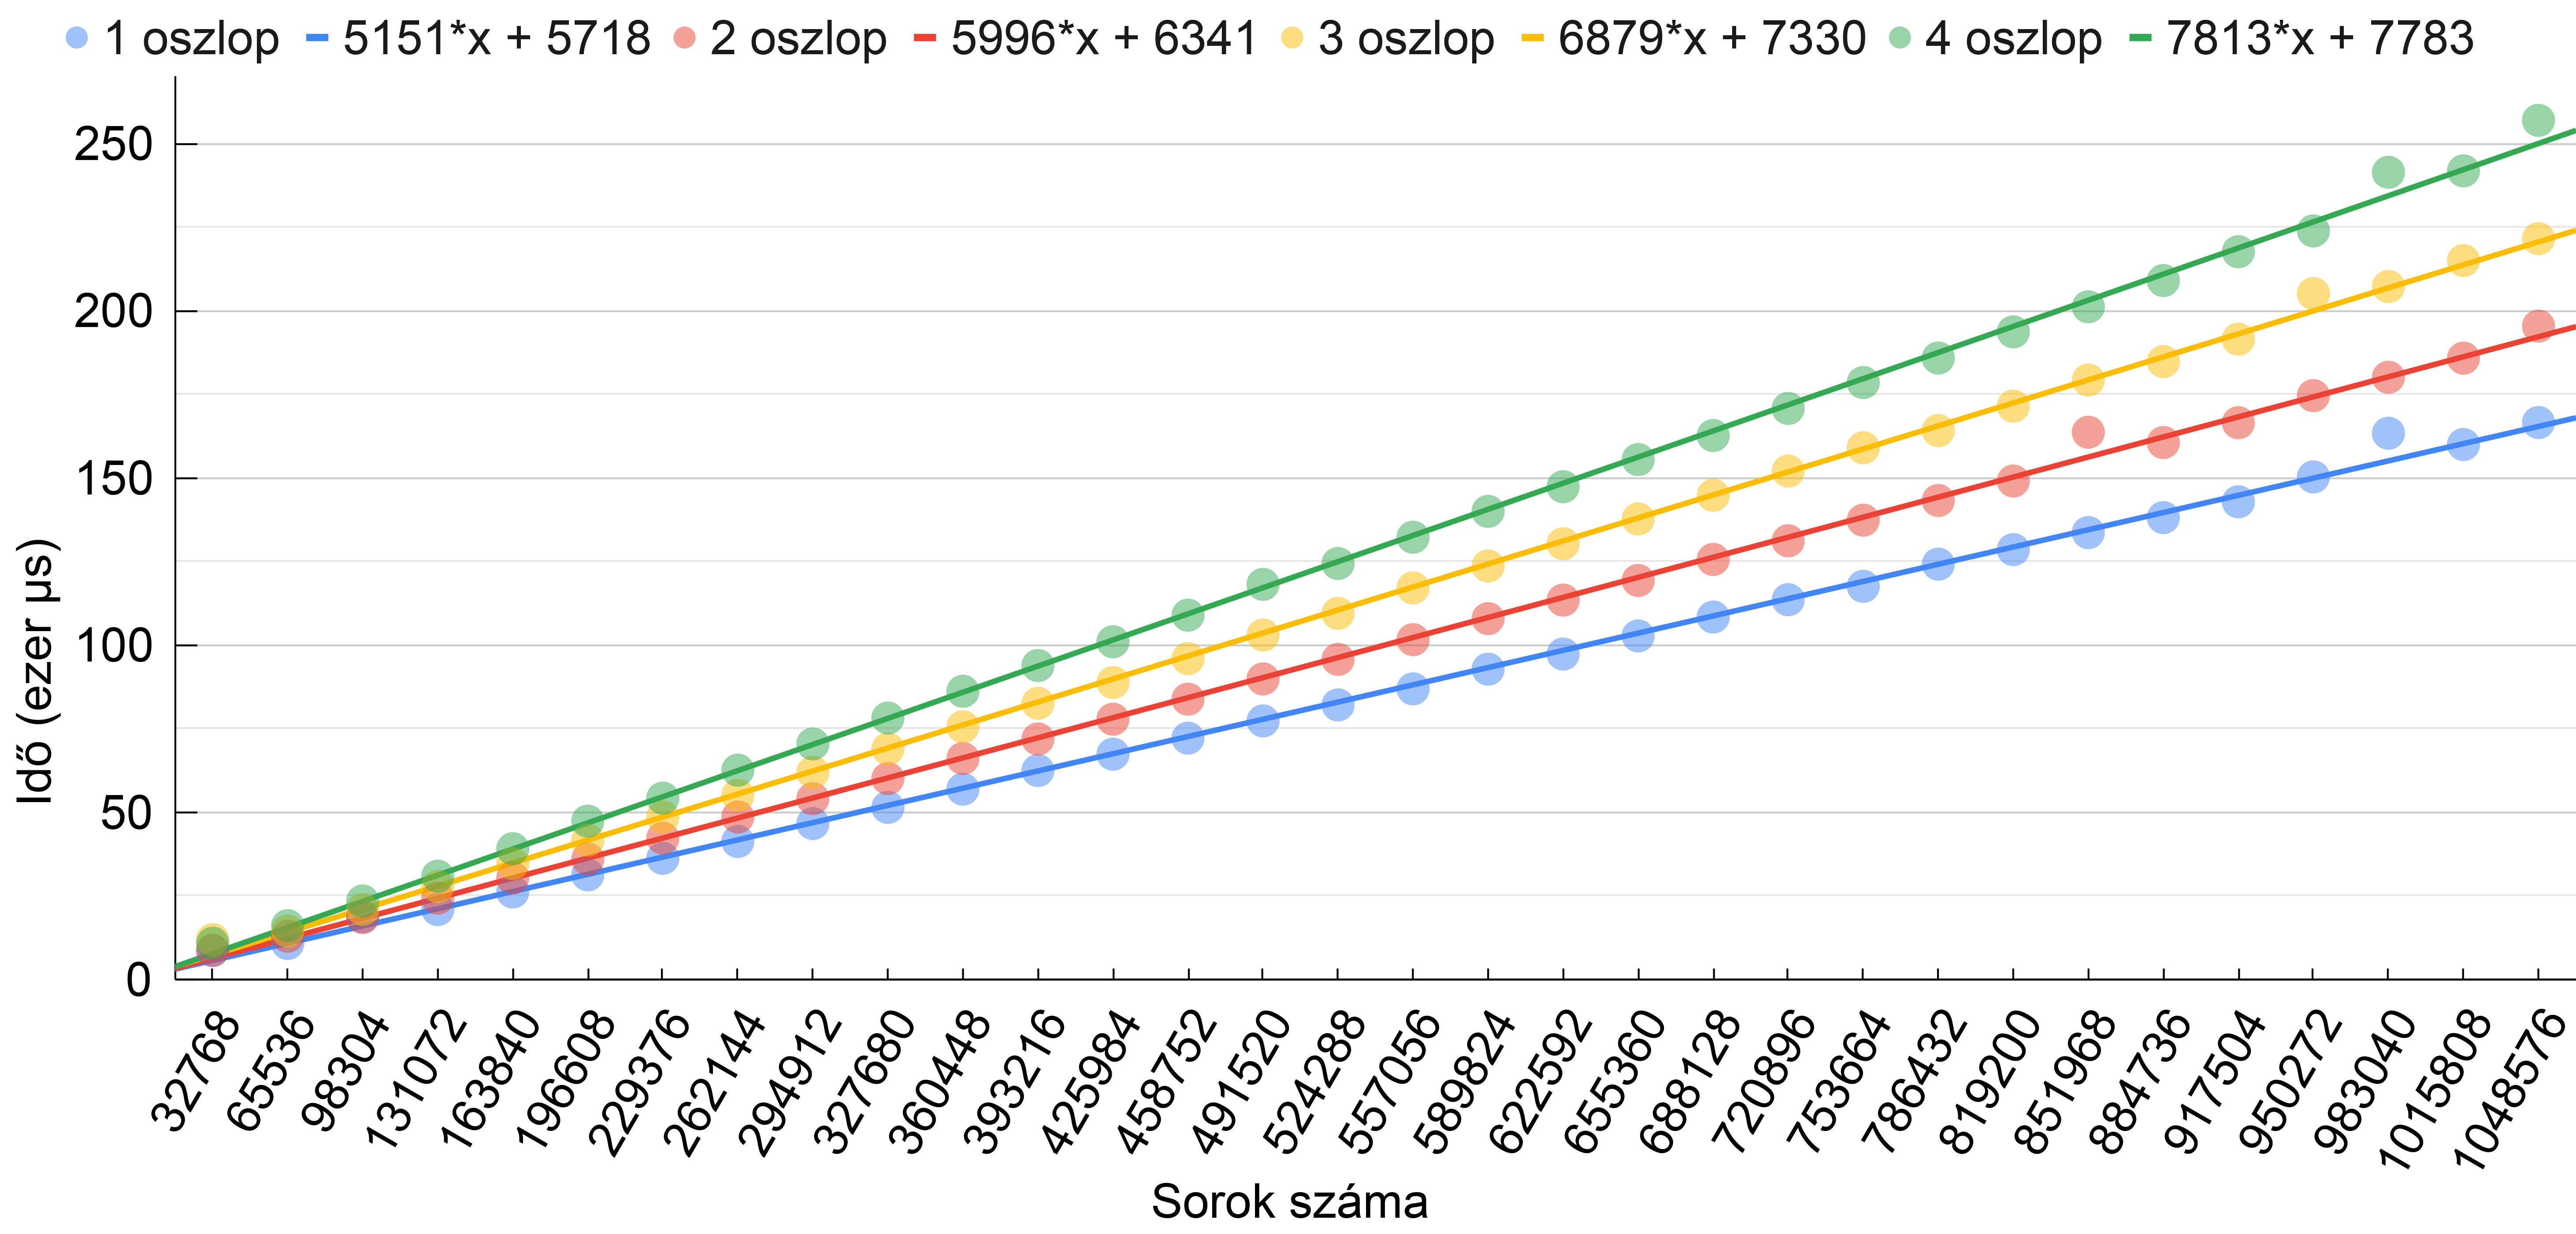
\includegraphics[width=\textwidth]{images/graph/sqlquery.png}
\caption{Az SQL lekérdezési sebessége}
\label{fig:sqlquery}
\end{figure}

\Aref{fig:sqlquery}. ábrán, egyértelműen látható, hogy a sorok számának növekedésével az idő is lineárisan nő.
A jelmagyarázatnál látható egyenes egyenletekből becsléseket lehet készíteni adott paraméterekkel rendelkező szűrés nélküli lekérdezéshez. 

Négy oszlop felett használjuk a 3 és 4 oszlop közötti növekedés mértékét, feltételezve, hogy innentől ez már nem változik. A kettő között eltérés lineáris becslésének képlete: 
$$7,79 \cdot 10^{-5} \cdot x + 1,13, \quad R^2=0,992,$$ 
ahol
$$x = \dfrac{\text{sorok száma}}{32768} - 1.$$
4 oszlop esetén:
$$ 7813 \cdot \text{sorok száma} + 7783 = \text{lekérdezés ideje}.$$

\SubSection{A query válaszának átmásolása a saját tömbbe}

A vizsgálathoz használt kód a programok \texttt{cp\_to\_array} nevű mappájában található.

A lekérdezésből kapott választ át kell másolni az általunk létrehozott tömbbe. Ez az egyik legköltségesebb művelet, ezért optimalizálásként itt is célszerű csak a felhasznált oszlopokat lekérni.
A mért program szakasz:
\begin{python}
int i = 0;
*T1_size = res->rowsCount();
*T1 = (Table1Type*) malloc(sizeof(Table1Type) * *T1_size);

while (res->next())
{
    T1[0][i].c1p1 = res->getInt("c1p1");
    // ...
    T1[0][i].c4 = res->getInt("c4");
    i++;
}
delete res;
delete pstmt;
\end{python}
Itt a válaszból lekérdezzük a méretet, majd ez alapján létrehozzuk a saját objektumunkat a memóriában, ezután egyesével belemásoljuk a kapott adatokat soronként.
Az mérési módszer megegyezik az előzőekben használtakkal.

\begin{figure}[h!]
\centering
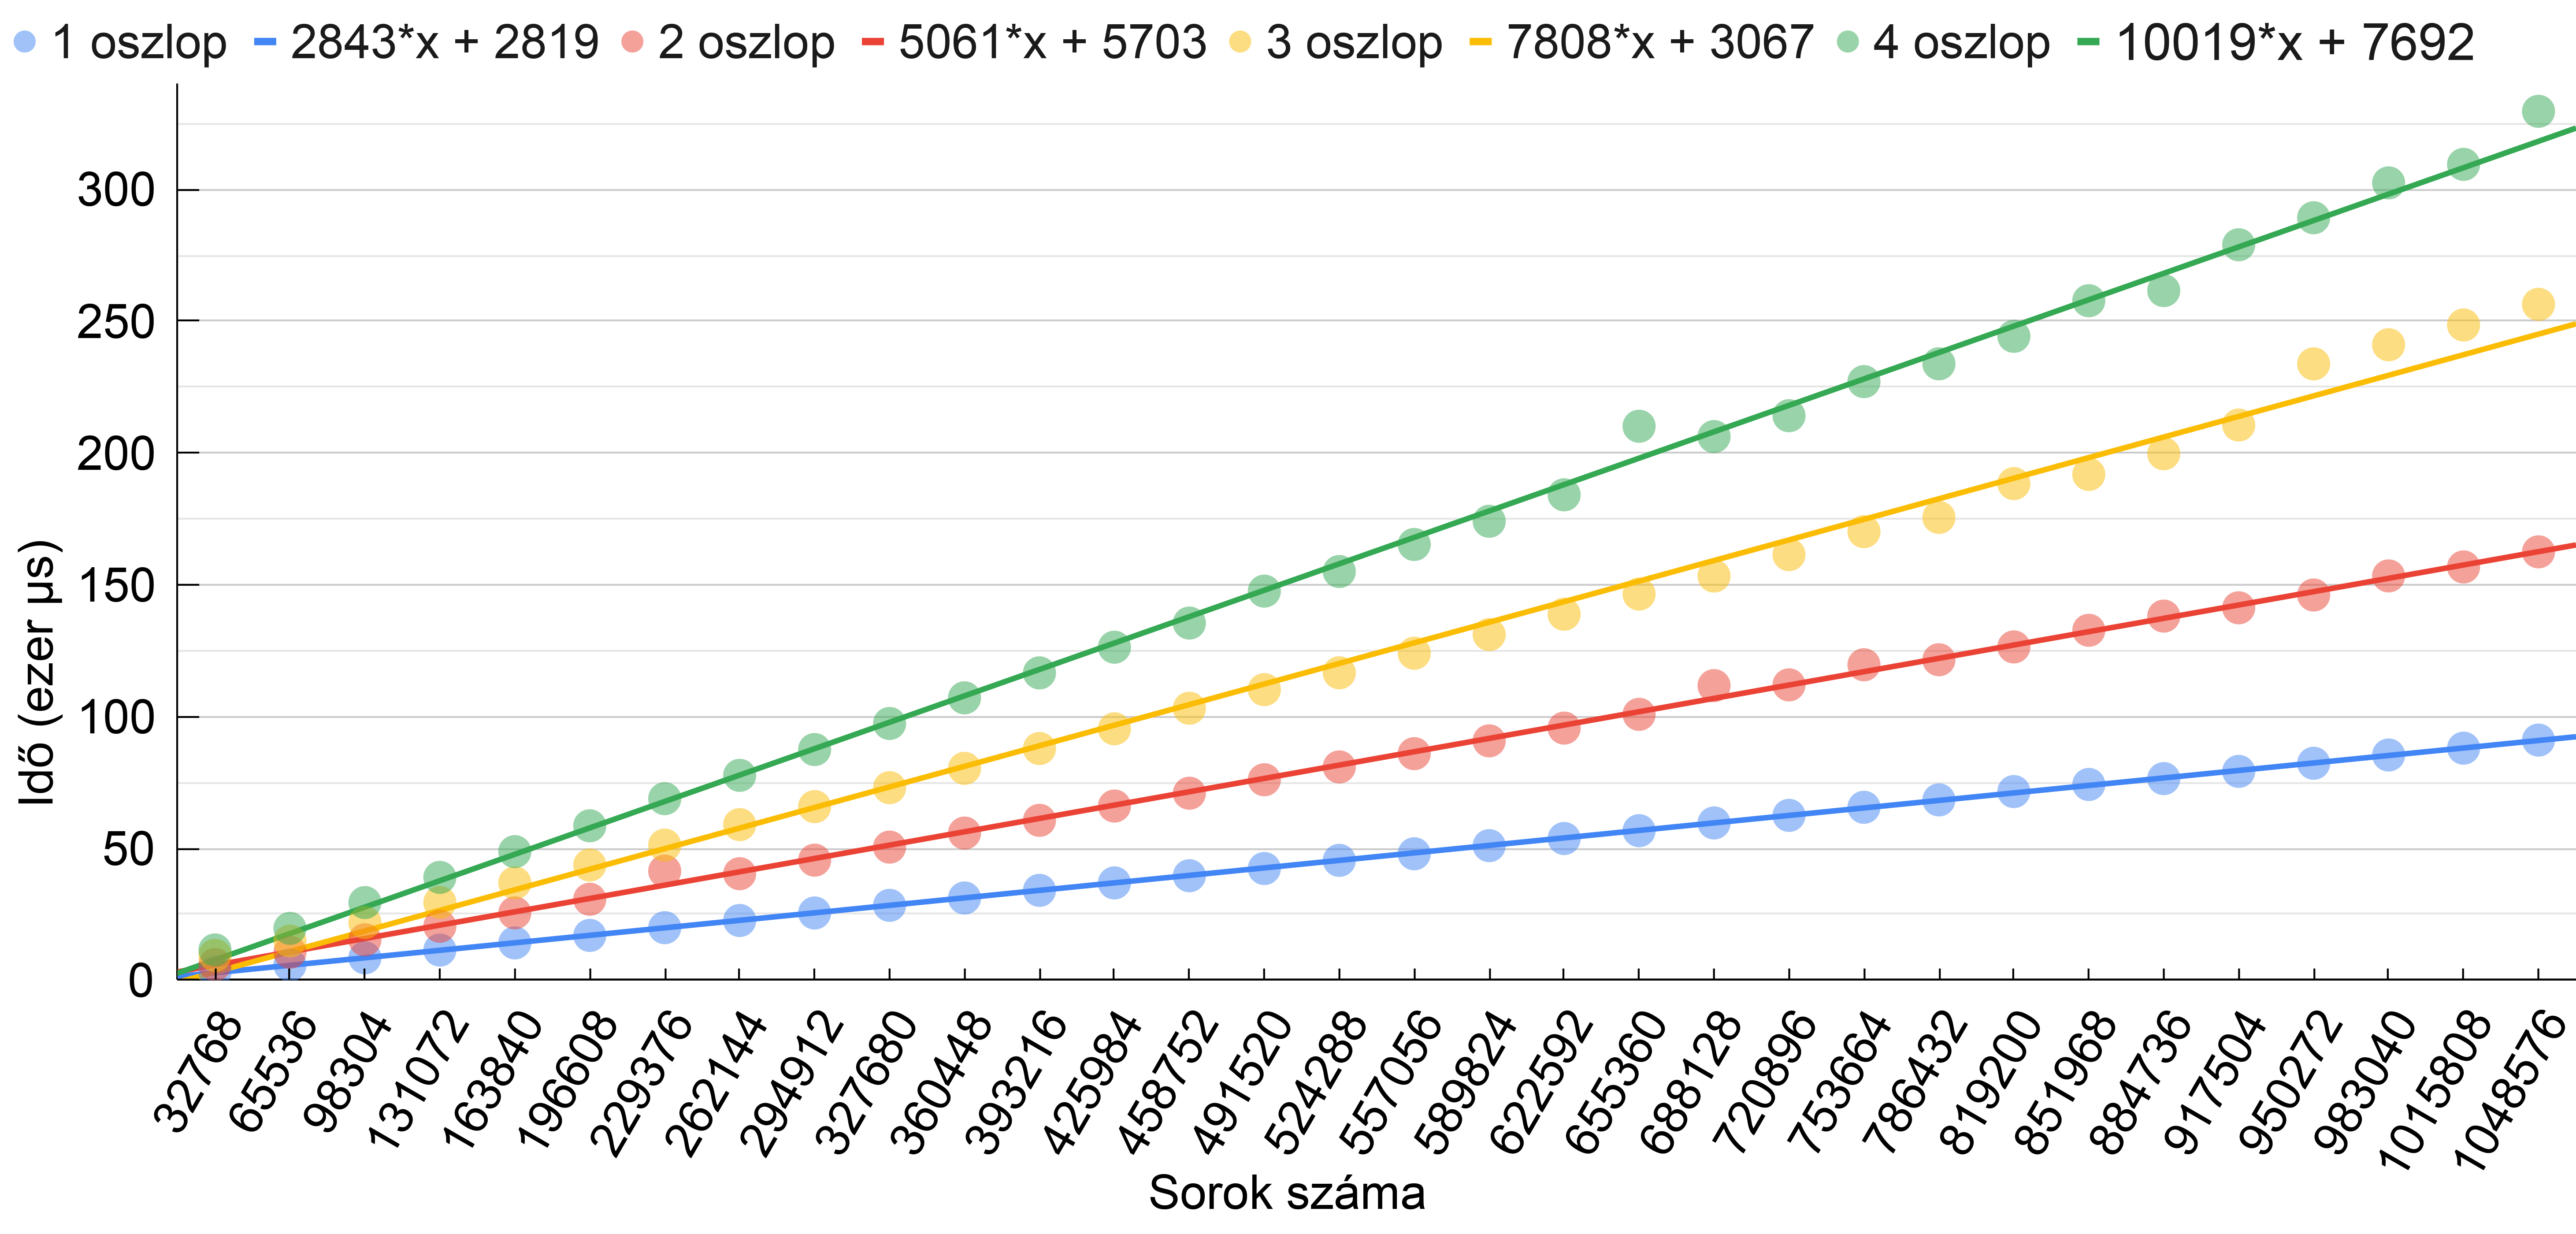
\includegraphics[width=\textwidth]{images/graph/ccopy.png}
\caption{Adatok másolása saját tömbbe}
\label{fig:ccopy}
\end{figure}

\Aref{fig:ccopy}. ábrán látható grafikonon két dolgot vehetünk észre azonnal. Az egyik az, hogy ez a folyamat lassabb mint maga a lekérdezés a másik pedig, hogy drasztikusabb a növekedés az oszlopok számának sokasodásával.
Tételezzük fel, csak úgy mint az előző esetben, hogy 4 oszlop felett nem több az elérés, mint 3 és 4 között.
A két oszlop közötti eltérés lineáris becslése:
$$-6,1 \cdot 10^{-4} \cdot x + 1,32, \quad R^2=0,99,$$ 
ahol
$$x = \dfrac{\text{sorok száma}}{32768} - 1.$$
Becslés 4 oszlop esetén:
$$ 10019 \cdot x + 7692 = \text{másolás ideje}$$

\SubSection{Adatok bemásolása a pufferekbe}

Az adatok átmásolása az OpenCL puffereibe szintén egy olyan része a programnak, ami sok időt emészthet fel.
(Az ehhez elkészített program neve \texttt{cp\_buffer}.)
Vizsgáljuk meg a következő kódrészt.
\begin{python}
int range = 65536;
while (range <= 1048576)
{
 clStatus = clEnqueueWriteBuffer(command_queue, Table1_clmem,
  CL_TRUE, 0, range * sizeof(Table1Type), t1, 0, NULL, NULL);
 clStatus = clEnqueueWriteBuffer(command_queue, Table_size_clmem,
  CL_TRUE, 0, sizeof(int), &t1_size, 0, NULL, NULL);
 clStatus = clEnqueueWriteBuffer(command_queue, Interval_size_clmem,
  CL_TRUE, 0, sizeof(int), &interval_size, 0, NULL, NULL);
 clStatus = clFinish(command_queue);
 range += 65536;
}
\end{python}

\begin{figure}[h!]
\centering
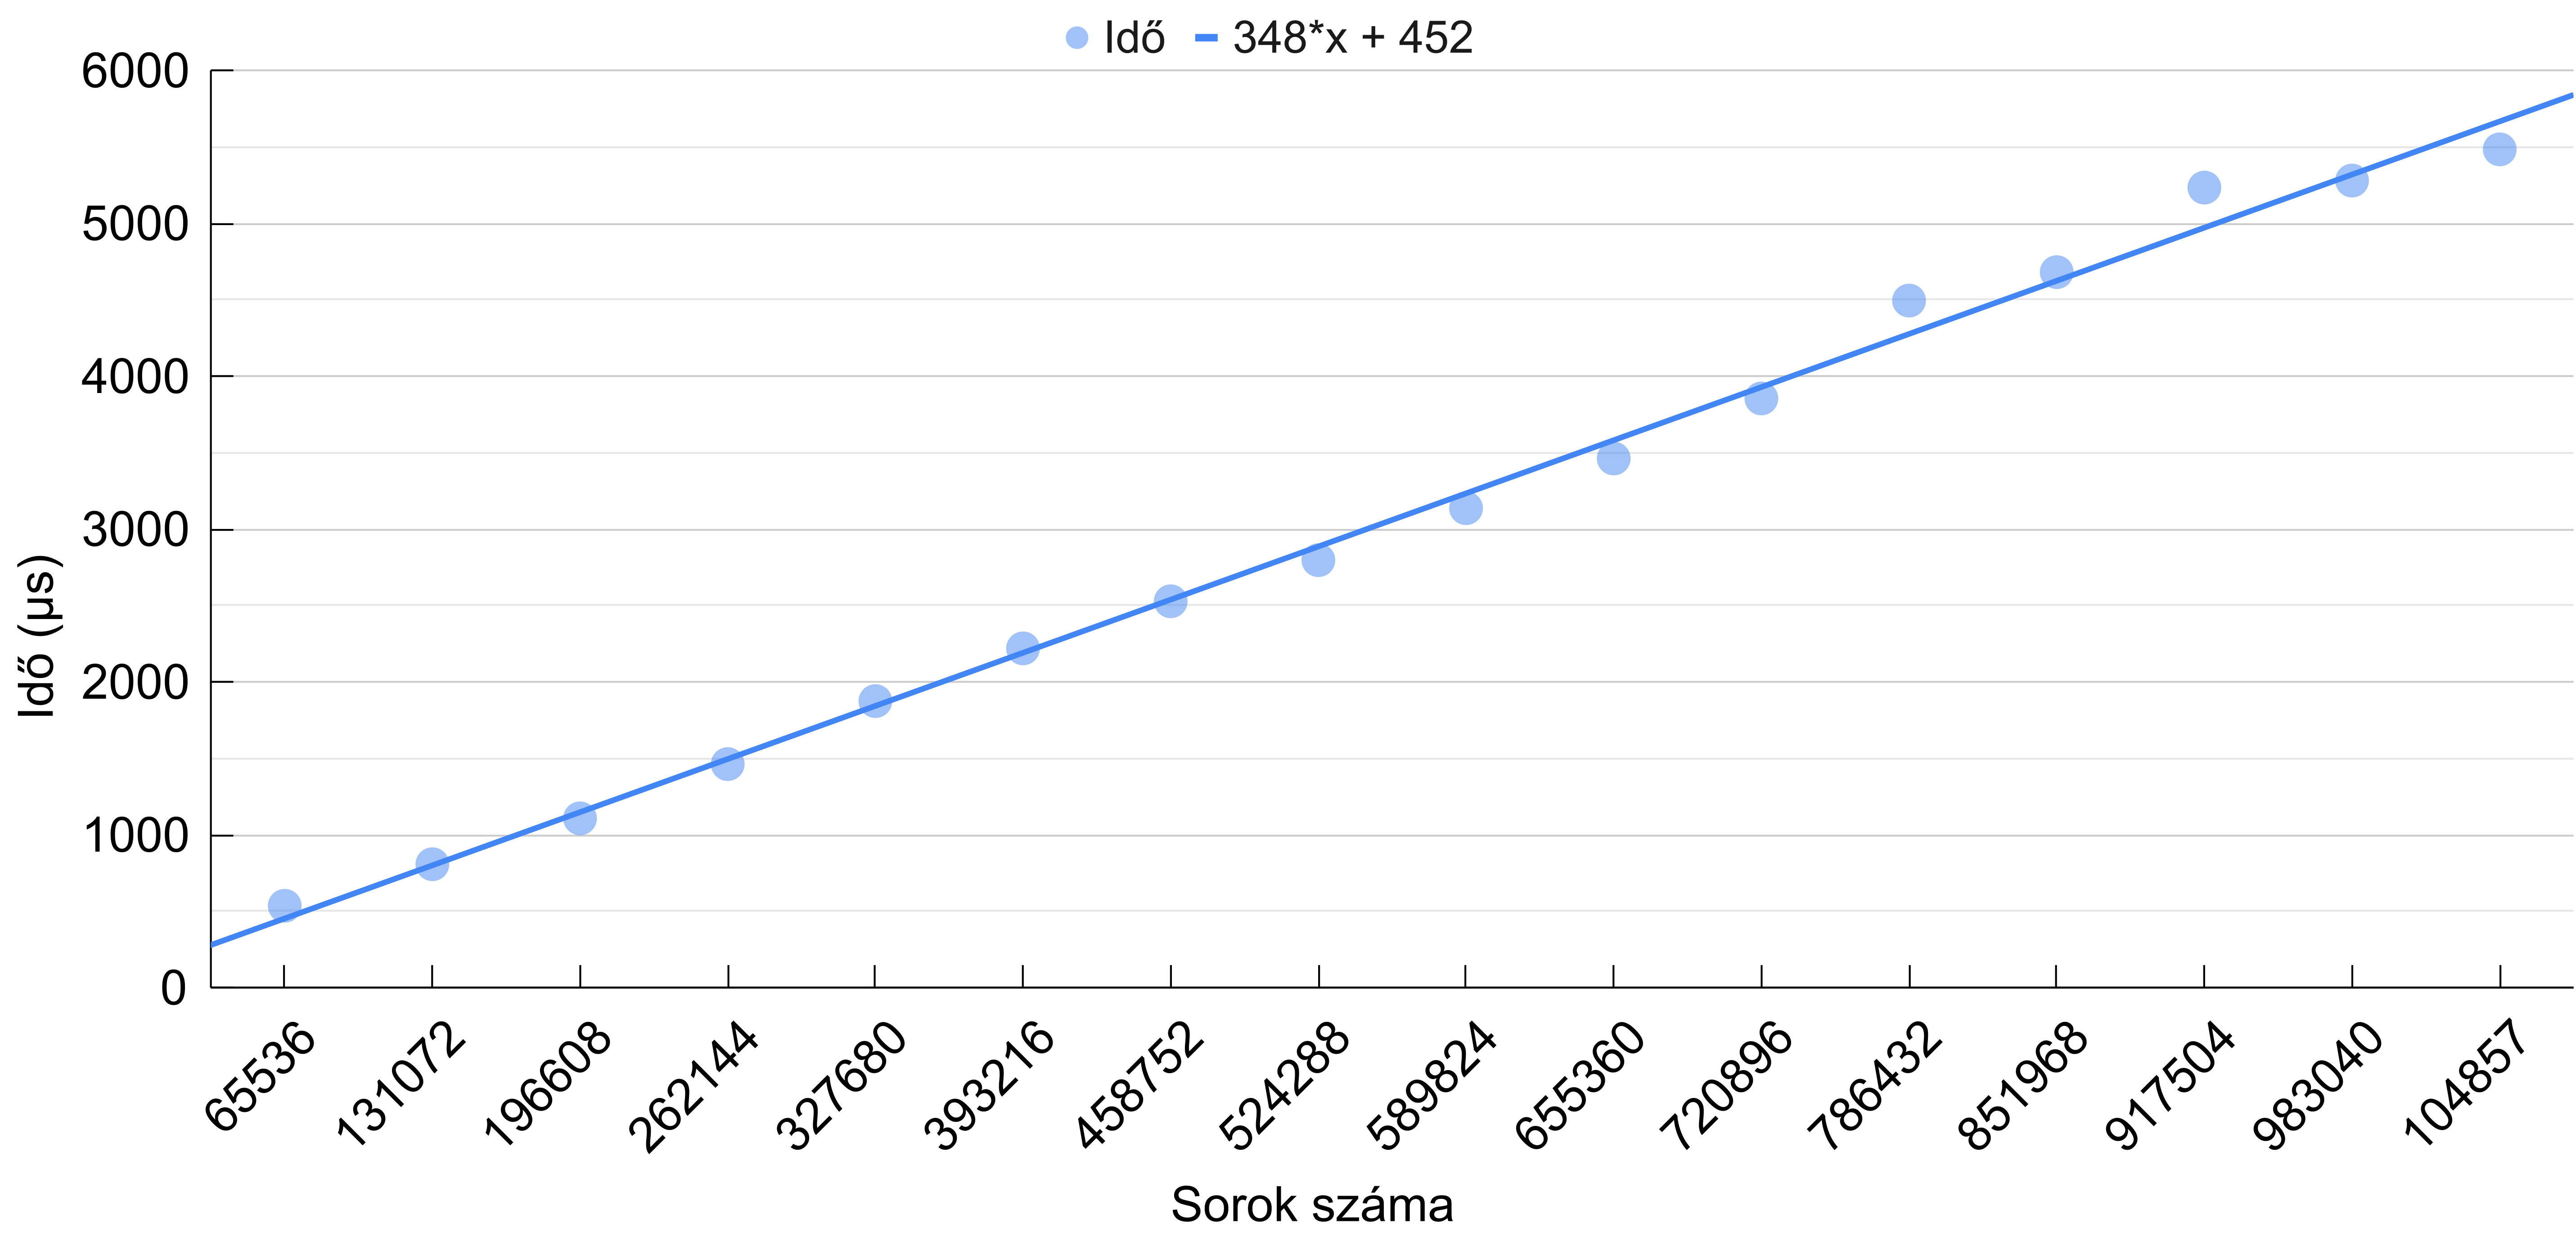
\includegraphics[width=\textwidth]{images/graph/pufferin.png}
\caption{Adatok bemásolása 2.}
\label{fig:pufferin}
\end{figure}

Mivel ebben az esetben a másolás egybefüggő memória területre vonatkozik, nem pedig elemenkénti hivatkozás, ezért elegendő egyetlen mérés.
\Aref{fig:pufferin}. grafikonon egy 4 oszlopos tábla átmásolásának a sebessége látható. Ebből több vagy kevesebb oszlopra, illetve sorra a becslés egyszerű szorzásokkal megkapható.

4 és 3 oszlop esetén:
$$ x = \text{sorok száma} / 65536, $$
$$ 348*x + 452 = \text{pufferbe másolás ideje}, $$ 
$$ \text{pufferbe másolás ideje} * 0.75 = \text{3 oszlopos pufferbe másolás ideje}. $$

\SubSection{Adatok kimásolása a pufferekből}

Nézzük az első kiolvasási módszert, amikor a teljes eredmény tömböt illetve a hozzá tartozó számlálót másoljuk ki.
Jelen mérésnél a lista csak egyetlen indexet tartalmaz:
$$ x = \text{sorok száma} / 65536, $$
$$ 81,2*x + 156 = \text{puffer kiolvasási ideje}. $$ 
Az előzőhöz hasonlóan itt is egy memória darabot másolunk, ennek szorzásával megkapjuk mennyi időbe telne a kiolvasás más méretek esetén (\ref{fig:pufferout}. ábra).

\begin{figure}[h!]
	\centering
	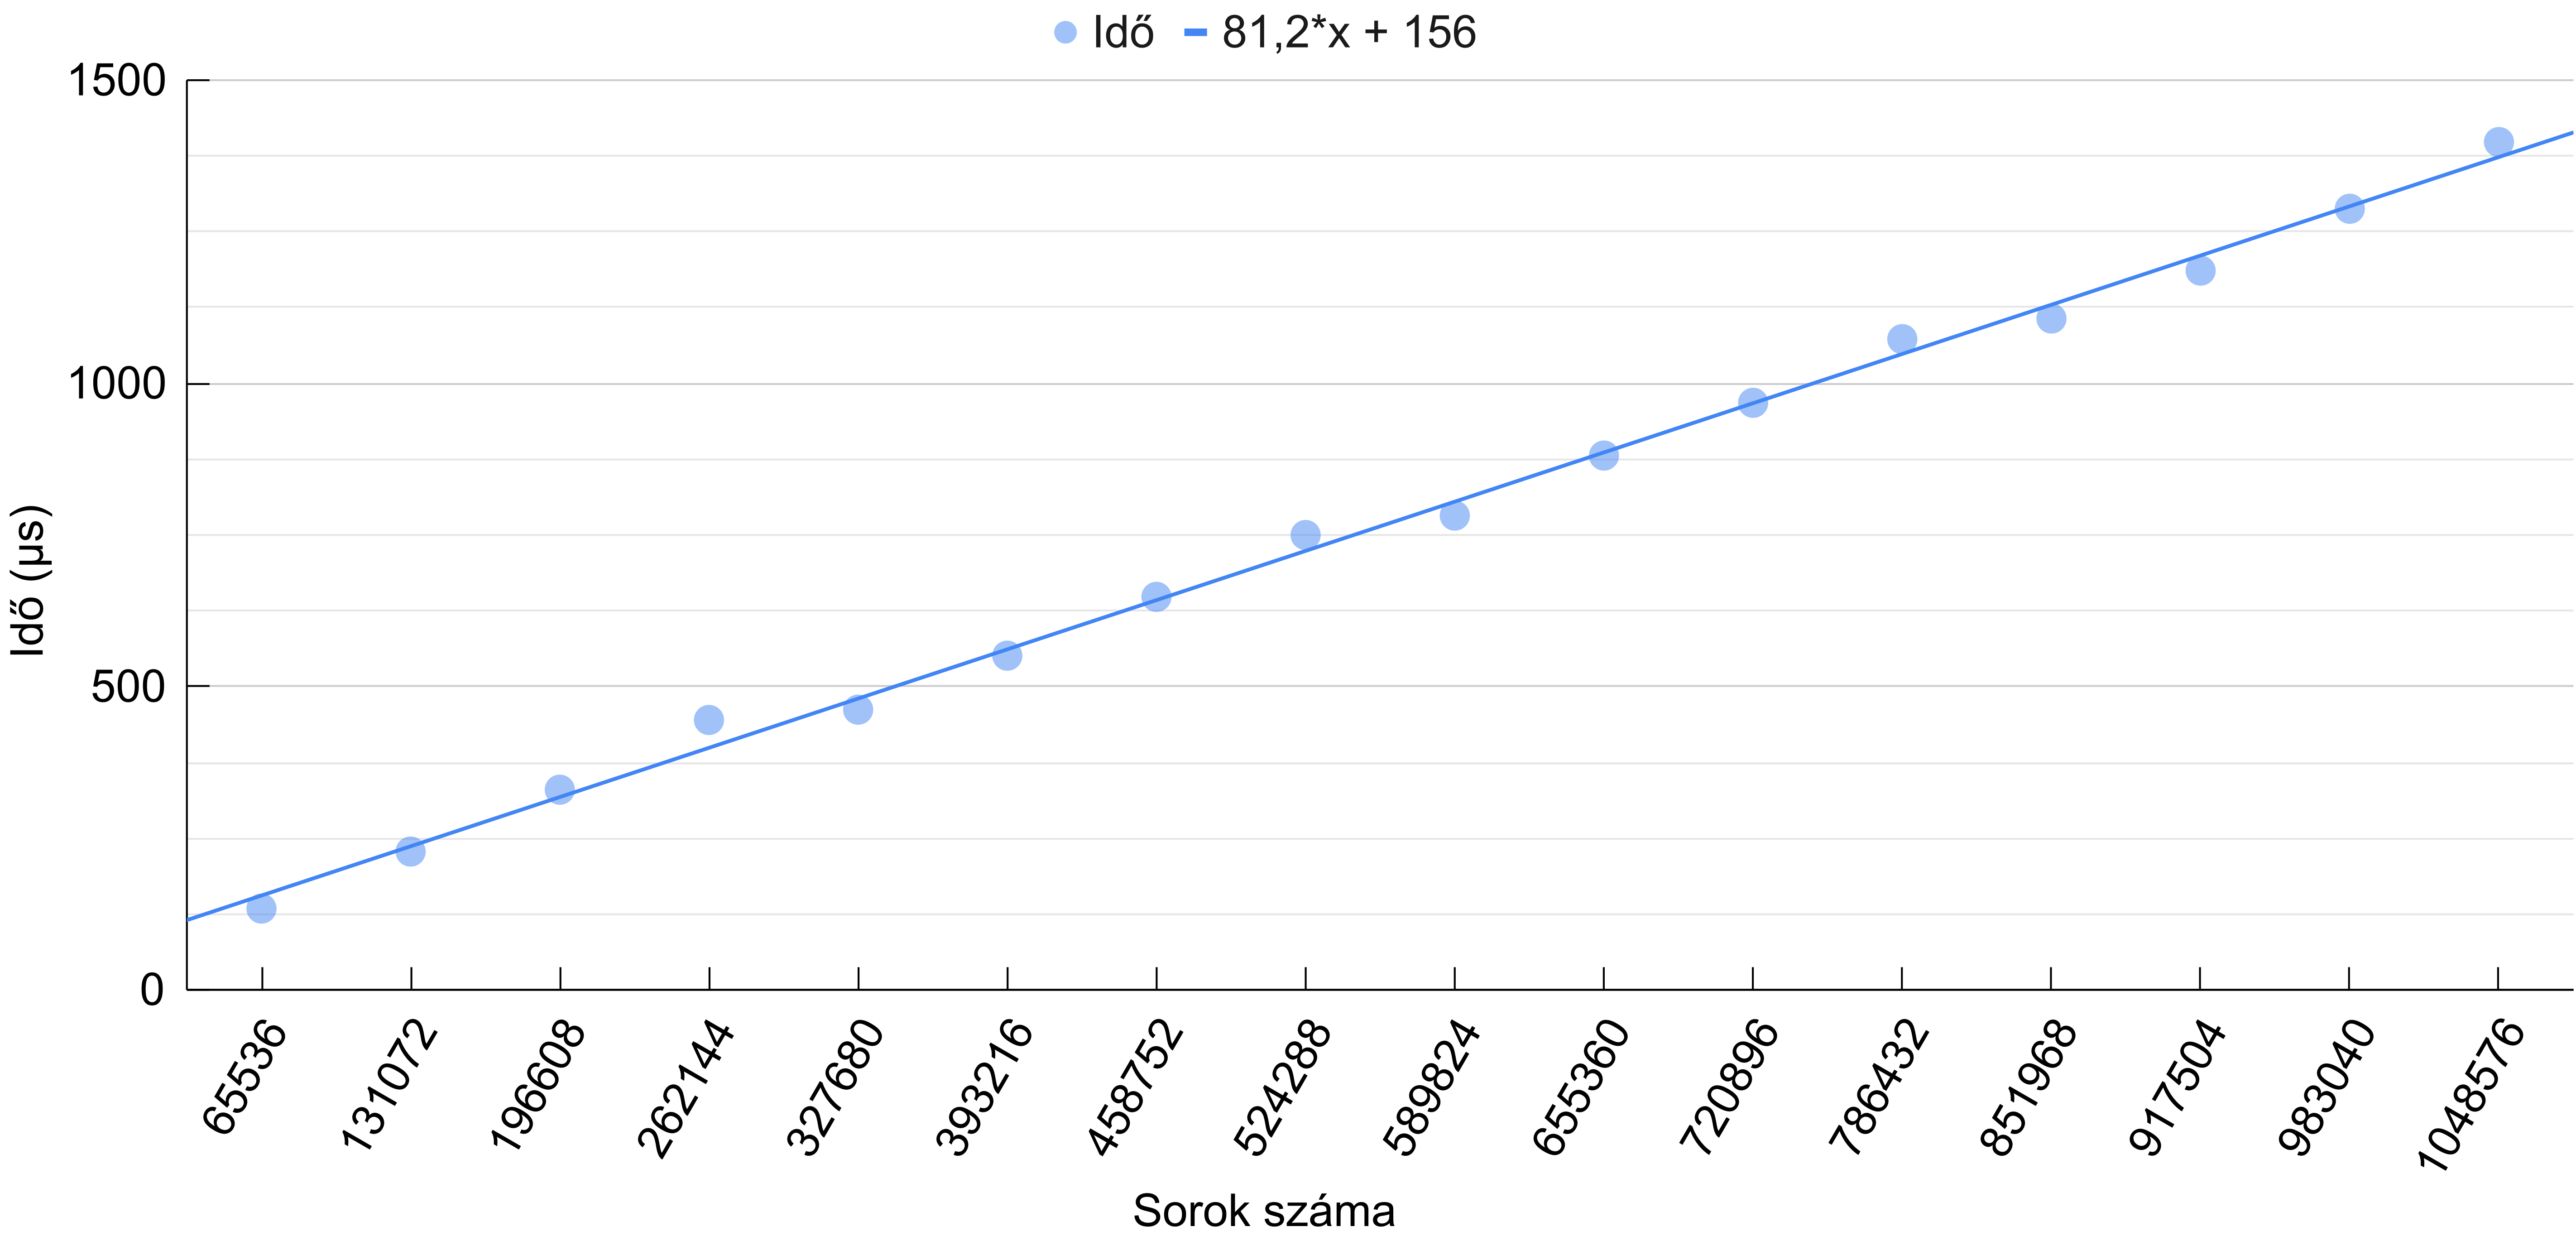
\includegraphics[width=14.8cm]{images/graph/pufferout.png}
	\caption{Adatok kimásolása 2.}
	\label{fig:pufferout}
\end{figure}

Fontos megjegyezni, hogy a mérések egy, program futtatáson belül történetek. Ez azért olyan lényeges, mert operációs rendszer és egyéb memória kezelési tényezők miatt, az első kimásolás akár 25\% al is lassabb lehet mint az azt követőek ugyan azon pufferből.

A másik módszer, miszerint nem olvassuk ki azonnal a teljes választ, hanem alkalmazzuk az előző fejezetben taglalt optimalizálási eljárást.
Ennek hatékonysága a sok kisebb olvasás miatt függ az eredmények számától. Ennek méréséhez módosítani kell a kernel kódot, ezért manuálisan végeztem a méréseket, vagyis a szűrési feltételeket úgy módosítottam, hogy a találatok száma megfelelően változzon.

\begin{figure}[h!]
\centering
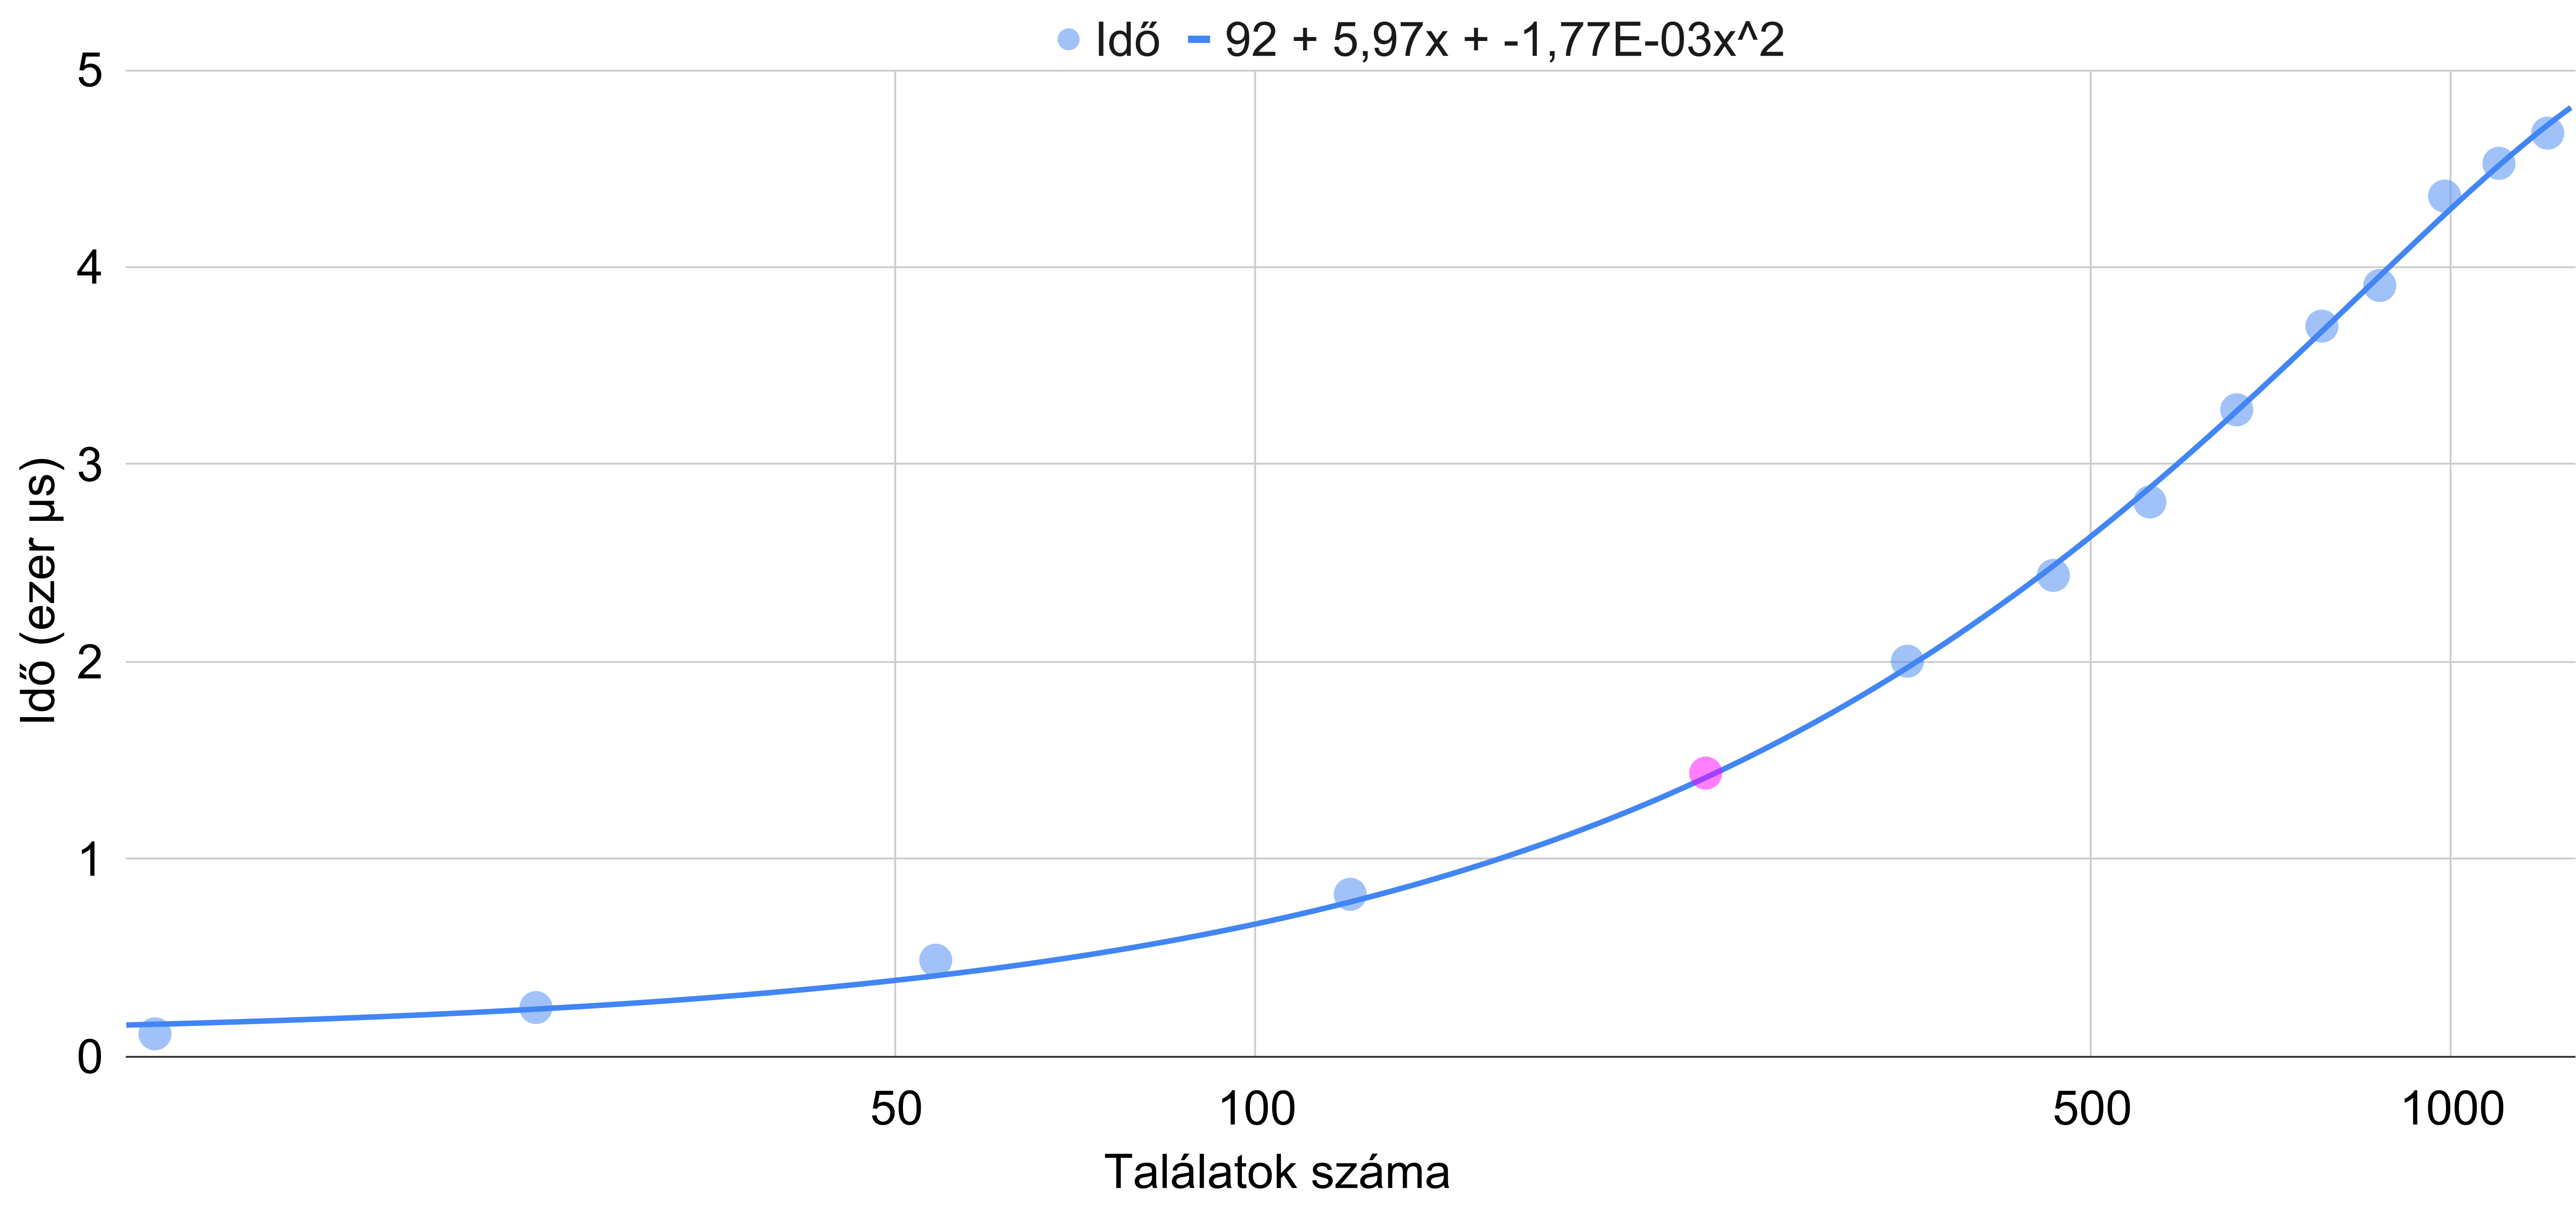
\includegraphics[width=14.8cm]{images/graph/outpuffer2_1.png}
\caption{Adatok kimásolása 2.}
\label{fig:outpuffer2_1}
\end{figure}

\begin{figure}[h!]
\centering
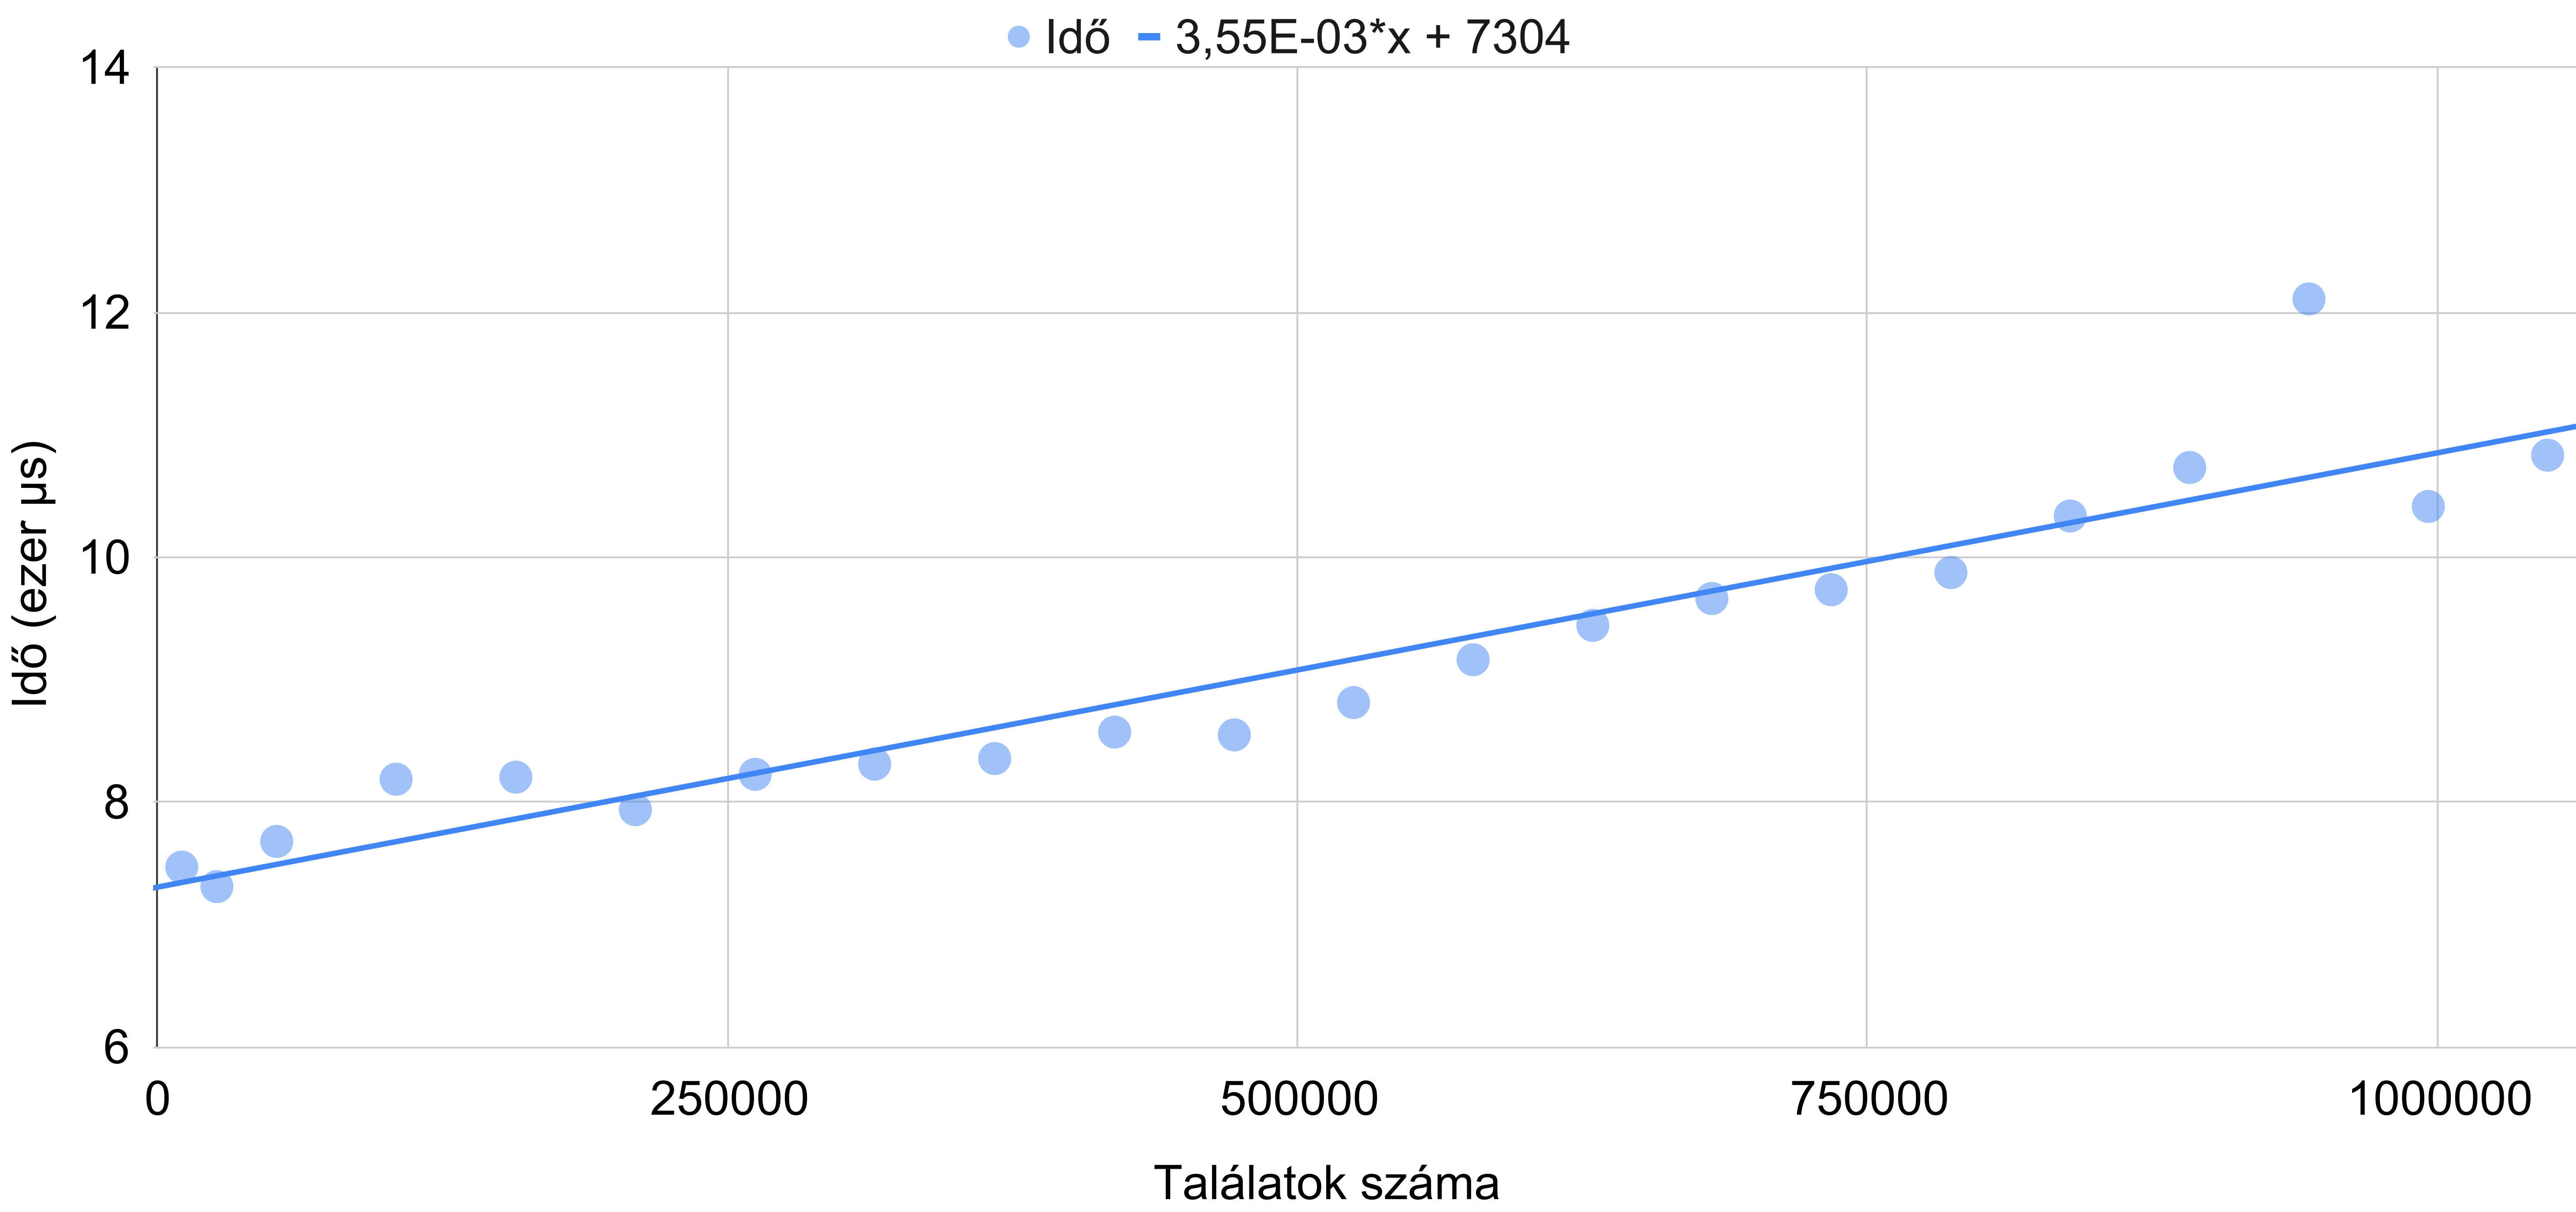
\includegraphics[width=14.8cm]{images/graph/outpuffer2_2.png}
\caption{Adatok kimásolása 2.}
\label{fig:outpuffer2_2}
\end{figure}

Végeredményként \aref{fig:outpuffer2_1}. és \aref{fig:outpuffer2_2}. ábrákon láthatjuk, hogy ez a fajta kiolvasás rendkívül hatékony, de csak abban az esetben, ha a találatok száma minimális.
238 találatnál a módszer elérte azt az időt, ami alatt el lehet végezni a teljes másolást egy darabban.

\SubSection{A globális méretből adódó sebességek}

A megfelelő globális méret meghatározása futási idő szempontjából nagyon fontos.

A túl nagy globális méret hatásai a következők.
\begin{itemize}
\item A lokális méret korlátai miatt túl sok csoport jön létre, így azok feldolgozása soros lesz.
\item A kimeneti számláló mérete megnő, ennek kiolvasása több idő, és alacsony találati szám mellett a fölösleges ellenőrzések száma szignifikáns lehet.
\end{itemize}

A túl alacsony globális méret hatásai pedig az alábbiak.
\begin{itemize}
\item A lokális méretet is szükséges lehet csökkenteni. Ha túl alacsony, akkor egyetlen munkaelem fogja végrehajtani, a párhuzamosság teljesen megszűnik.
\item A kimeneti számláló mérete alacsony, kevés visszatérő értéknél a kiolvasás gyors.
\end{itemize}
A méréseket ezen pontok alapján a következők szerint végeztem.
A globális méret változzon $[1, 2^{20}]$ tartományon, a lokális pedig $[1, 1024]$ tartományon négyzetes lépcsőkkel, az oszthatóságra figyelve.

A Gantt diagramhoz \texttt{ganttt}, a további grafikonokhoz tartozó pedig \\
\texttt{global\_size\_speed} néven szerepel az elkészített programok között. Nézzük meg ezek működését!
\begin{python}  
timer.start();

clStatus = clEnqueueNDRangeKernel(command_queue, kernel, 1, NULL, 
	&global_size, &local_size, 0, NULL, NULL);

clStatus =
	clEnqueueReadBuffer(command_queue, Result_indexes_list_clmem, 
	CL_TRUE, 0, global_size* sizeof(int), 
	result_counter, 0, NULL, NULL);
	
clStatus = clEnqueueReadBuffer(command_queue, TableResult_clmem, 
	CL_TRUE, 0, t1_size * sizeof(TableResultType), 
	result, 0,NULL, NULL);

clStatus = clFinish(command_queue);
clStatus = clFlush(command_queue);

for(int i=0; i<global_size; i++)
{
    for (int j = 0; j < result_counter[i]; j++ );
}
myfile << timer.elapsedMicroseconds() << ",";  
\end{python}

Szembetűnő lehet az egymásba ágyazott két ciklus. Azért szerepel ez kódrészlet a mérésekbe, hogy az eredményeken való végiglépegetés idejének nagyságrendje valamilyen módon meghatározható legyen. Fontos megjegyezni, hogy a fordítás során nem kerül figyelmen kívül hagyásra ez a két ciklus.

\Aref{fig:gantt}. ábrán látható Gantt-diagram mutatja részletesen, hogy mely program szakasz mennyi időbe telik.
Minden esetben a Lokális méret 32 és a visszatérő értékek száma körülbelül $50\%$, az eredményben pedig csak az index szerepel.

\begin{figure}[h!]
\centering
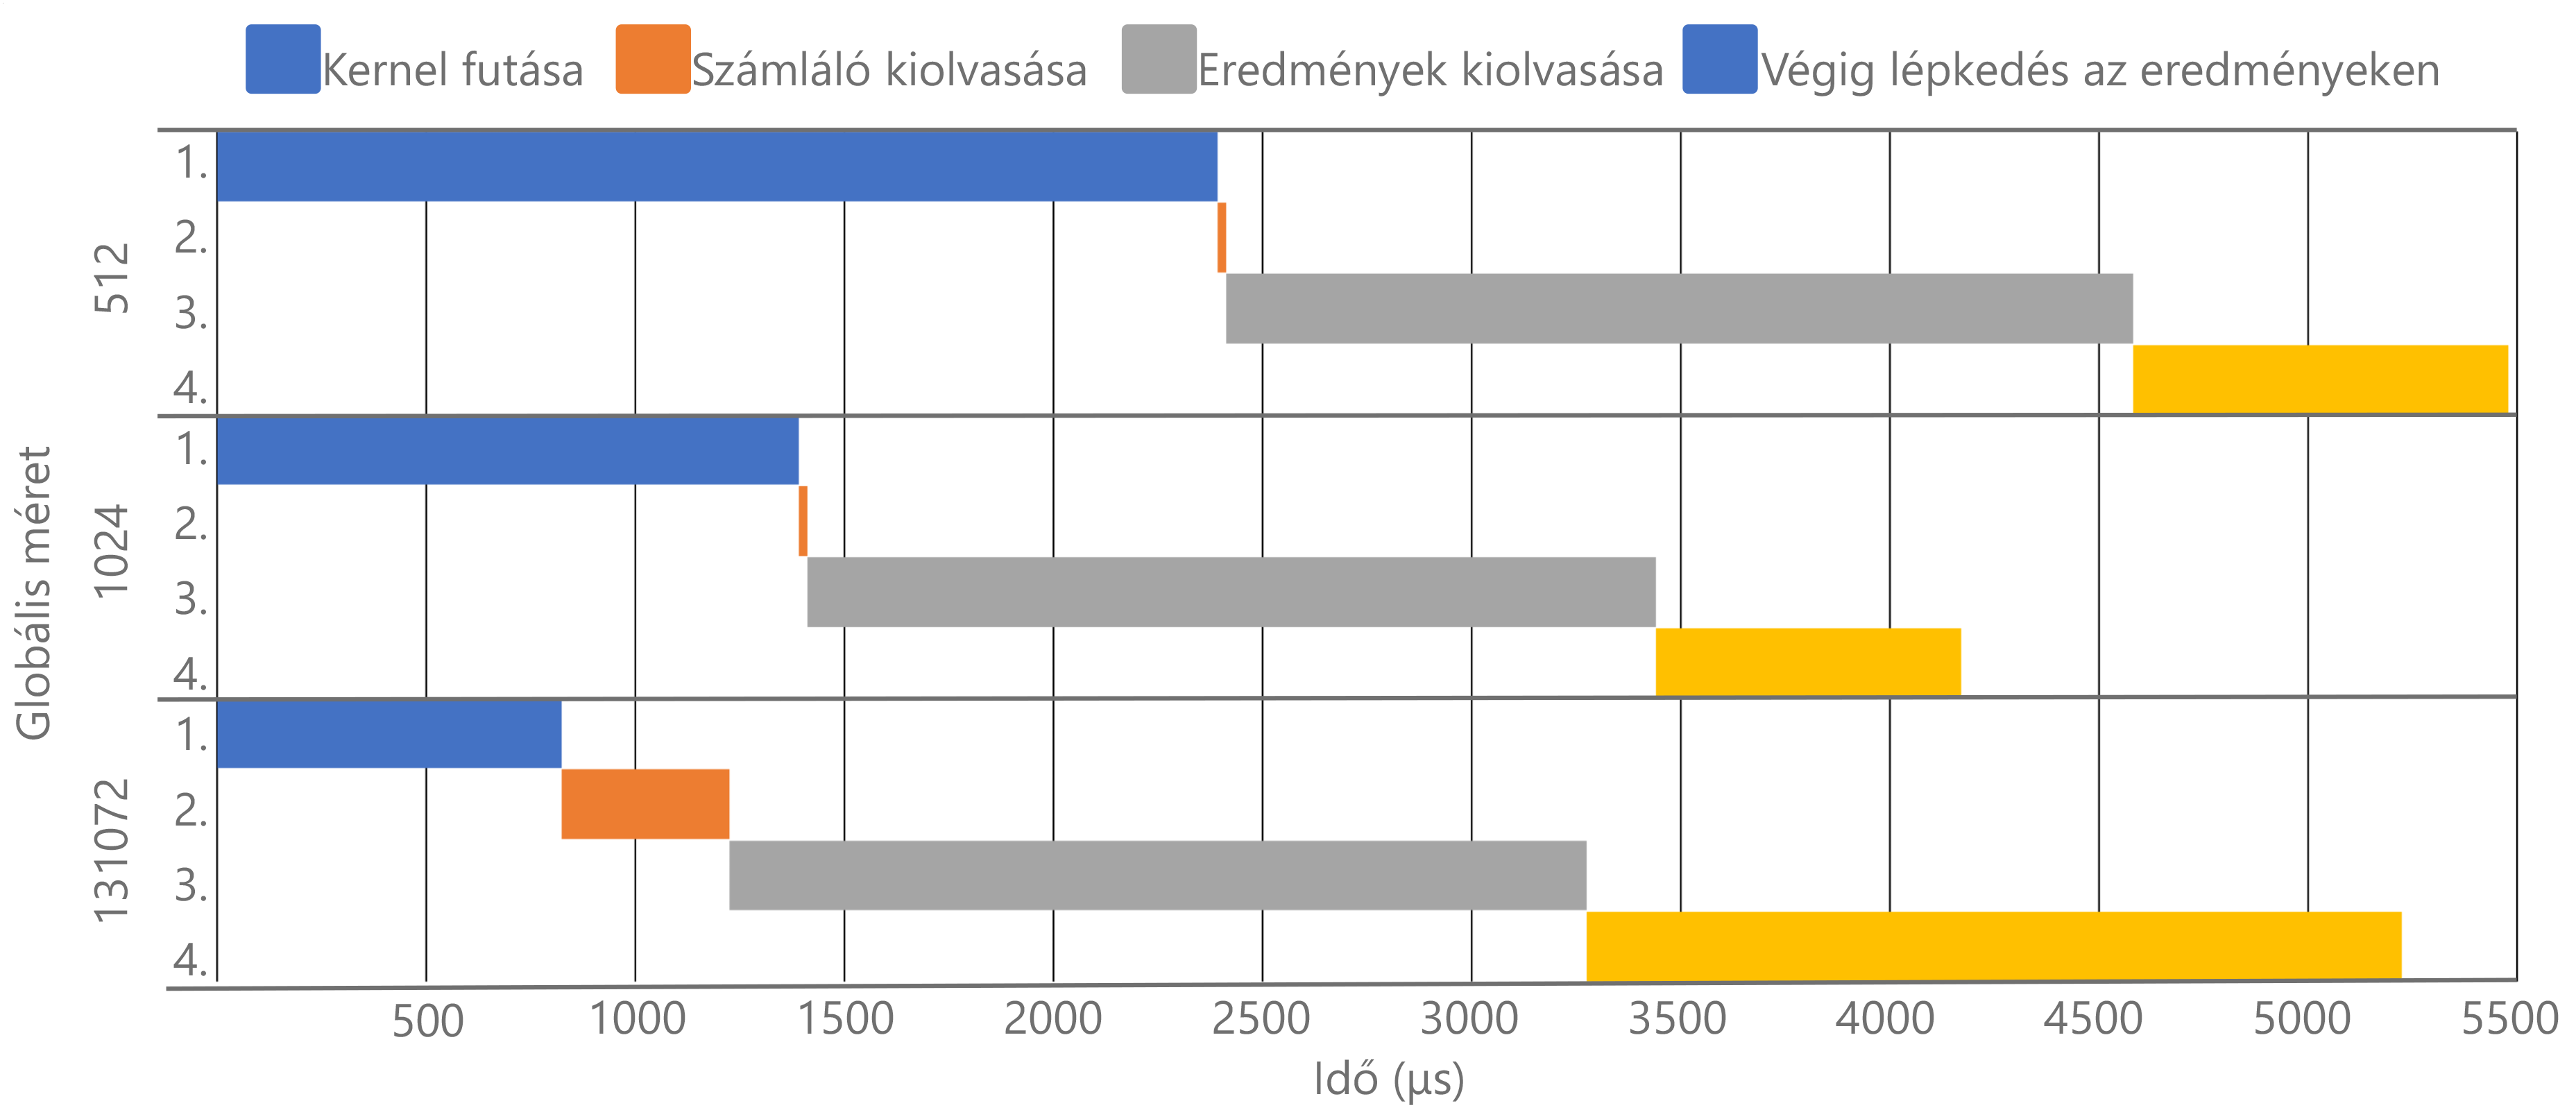
\includegraphics[width=\textwidth]{images/gantt.png}
\caption{Programszakaszok ideje.}
\label{fig:gantt}
\end{figure}

Látható, hogy a túl alacsony globális méret túl magas kernel futási időt eredményez. Túl nagy méret esetében pedig az eredmények kezelésének ideje válik számításigényessé.

(A diagram előállításához használt kód megtalálható a programok, \texttt{gantt} nevű mappában.)

\begin{figure}[h!]
\centering
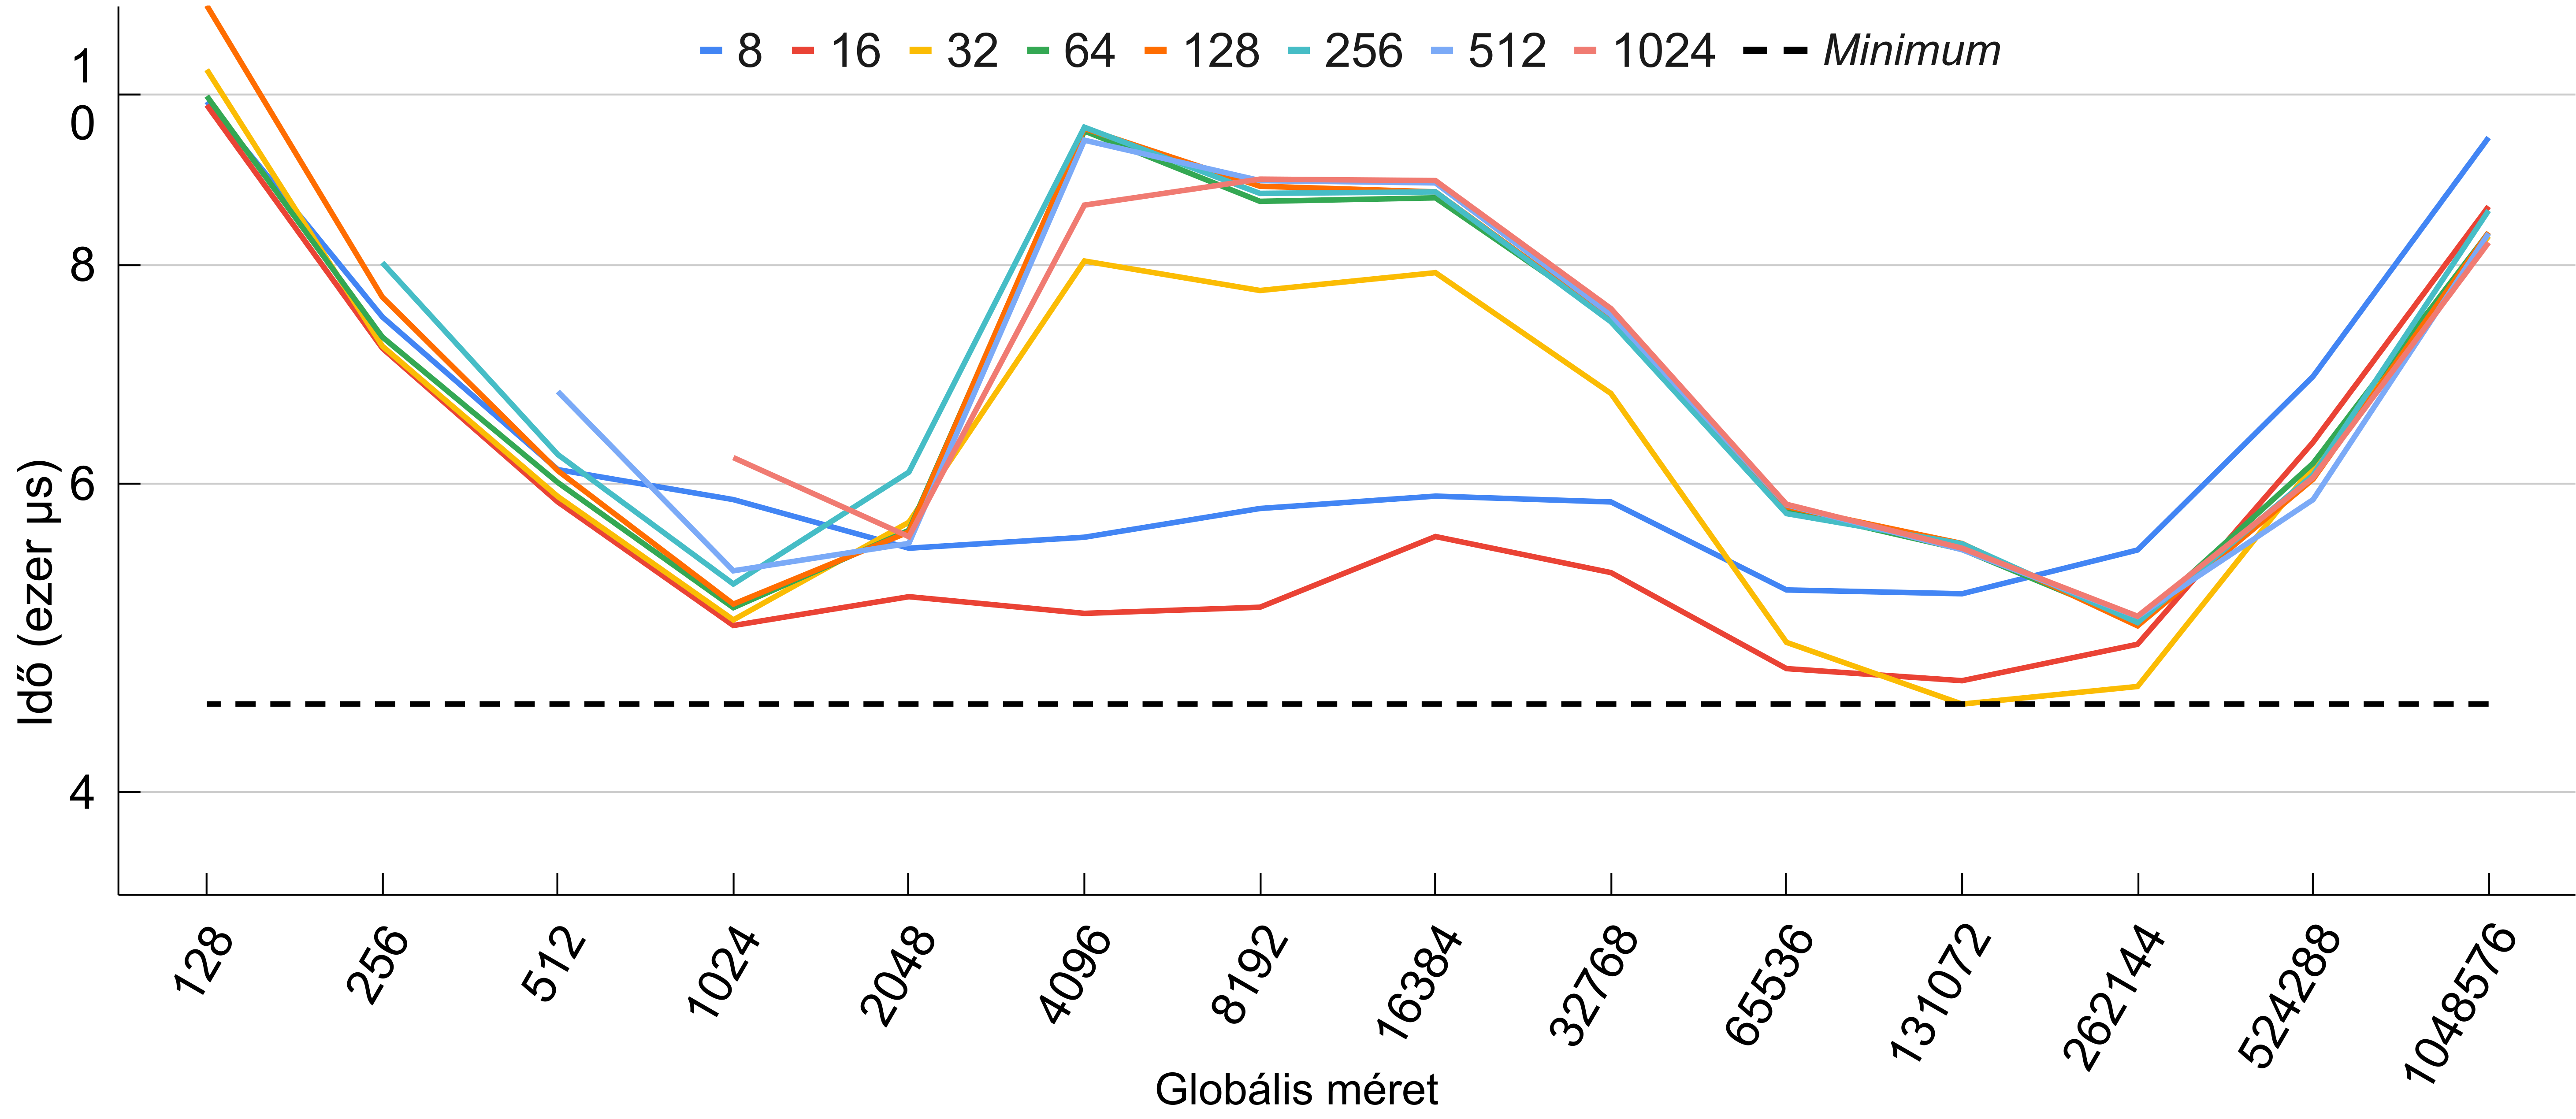
\includegraphics[width=\textwidth]{images/graph/global_size_1.png}
\caption{Maximális találat, az eredmény csak index.}
\label{fig:global_size_1}
\end{figure}

Az eredményt megvizsgálva látható, hogy van egy optimális globális méret tartomány $262144$ és $1024$ között (\ref{fig:global_size_1}. ábra).
Azt is észrevehetjük, hogy bizonyos lokális méretek ebben a tartományban drasztikusan rosszabb eredményt mutatnak.
A 16 és 32 -es méretek állnak legközelebb az ideális futási időhöz.

\begin{figure}[h!]
\centering
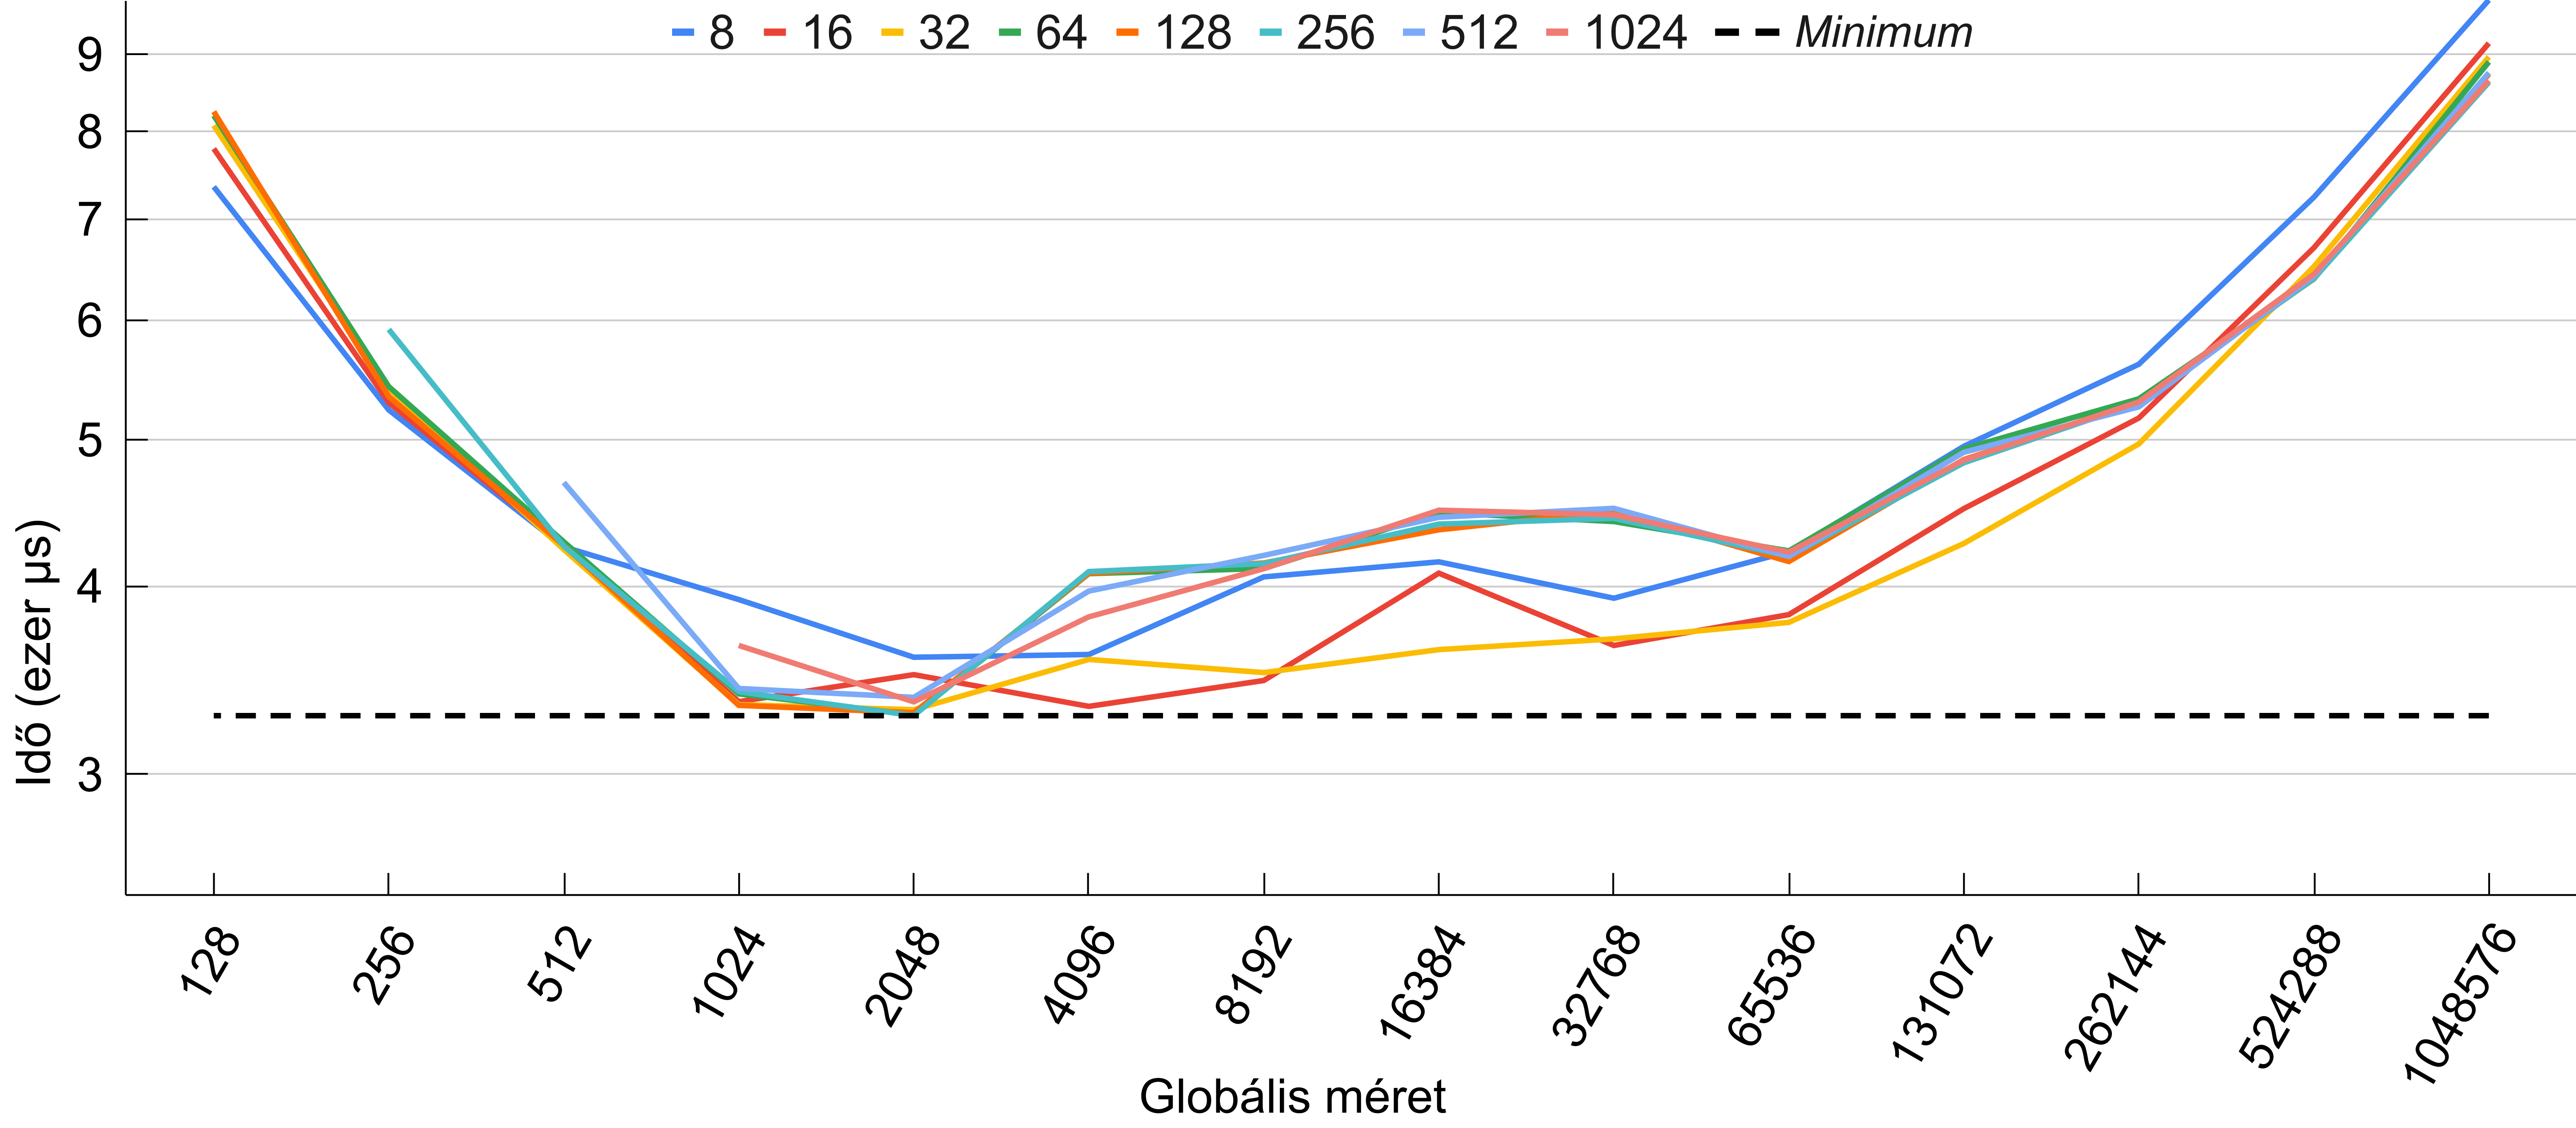
\includegraphics[width=\textwidth]{images/graph/global_size_2.png}
\caption{kb. 10\% találat, az eredmény csak index.}
\label{fig:global_size_2}
\end{figure}

\Aref{fig:global_size_2}. grafikonon egy olyan mérés látható, ahol a kernelben található feltételt úgy állítottam be, hogy megközelítőleg csak a tábla méretének 10\% -ával térjen vissza a lekérdezés.
Azt láthatjuk, hogy az előző középen lévő hullám lesimul, ez részben annak köszönhető hogy a kernel futási ideje csökken azzal, hogy nem kell annyi indexet az eredmény tömbbe írnia.

Azoknál a lekérdezéseknél, a kernelnek nem csak egy indexszel kell visszatérnie hanem több kalkulált értékkel is, ott is hasonló grafikonokat kapunk. De a kernel növekvő munkája és a megnövekedett adatmennyiség kiolvasása miatt a középen lévő hullám nagyobb és nehezebben lapul le.

Ezek alapján azt mondhatjuk, hogy közel ideális választás volt az 1024 mint globális méret.

\Section{Gyakorlati példák és következtetések}

A hatékonyság megállapításához a \textit{A MySQL lekérdezés sebessége} részben használt módszert fogom alkalmazni.
A fejezetben előfordulnak rövidítések: CONN - a MySQL Connector programra a CL pedig az OpenCL -t használó programra utal. 
A k betű ezres szorzót, az i betű pedig indexelés használatot jelöl.
\newline Bontsuk az \texttt{OpenCL} programot négy részre:
\begin{itemize}
\item Előkészítés - Minden ami a kernel futása előtt történik,
\item Kernel(ek) futása,
\item Eredmények kiolvasása,
\item Eredmények kezelése.
\end{itemize}
A \texttt{Connector} programot pedig 3 részre:
\begin{itemize}
\item Előkészítés - Minden ami a kernel futása előtt történik,
\item Lekérdezés - A korában már említett két sor,
\item Eredmények kezelése.
\end{itemize}
Az eredmény kezelése résznél azt vizsgáljuk melyik esetben gyorsabb az eredményeket fájlba írni.

\SubSection{Egy táblás lekérdezés}

(Forrás: programok, \texttt{program\_test}, \texttt{where} mappa.)

\begin{python}
SELECT * FROM speedtest_1048576 WHERE c3 = 1 AND c4 > 5001;
	5307 row(s) returned
SELECT * FROM speedtest_1048576 WHERE c3 > 1 AND c4 > 5001;
	514025 row(s) returned
\end{python}
Először vizsgáljuk meg azt, mennyi ideig tart a lekérdezés, ha a Connenctor-t használjuk.

\begin{table}[h!]
\centering
\begin{tabular}{|p{6cm}|p{3cm}|p{3cm}|}
\hline
Sorok száma & 5307 & 514025 \\
\hline\hline

Előkészítés & 21237 $\mu s$ & 19125 $\mu s$ \\
\hline

Lekérdezés & 183674 $\mu s$ & 273130 $\mu s$ \\
\hline

Eredmény kiírás & 12591 $\mu s$ & 1110877 $\mu s$ \\
\hline
\end{tabular}
\end{table}

\noindent Ugyanez indexeléssel:

\begin{table}[h!]
\centering
\begin{tabular}{|p{6cm}|p{3cm}|p{3cm}|}
\hline
Sorok száma & 5307 & 514025 \\
\hline
\hline

Előkészítés & 21483 $\mu s$ & 16573 $\mu s$ \\
\hline

Lekérdezés & 23979 $\mu s$ & 268184 $\mu s$ \\
\hline

Eredmény kiírás & 17009 $\mu s$ & 1087573 $\mu s$ \\
\hline
\end{tabular}
\end{table}

\newpage

\noindent Illetve az \texttt{OpenCL} program használatakor:

\begin{table}[h!]
\centering
\begin{tabular}{|p{6cm}|p{3cm}|p{3cm}|}
\hline
Sorok száma & 5307 & 514025 \\
\hline
\hline
Előkészítés & 692705 $\mu s$ & 682227 $\mu s$ \\
\hline
Kernel futás & 1129 $\mu s$ & 1602 $\mu s$ \\
\hline
Eredmény kiolvasás & 2197 $\mu s$ & 2013 $\mu s$ \\
\hline
Eredmény kiírás & 11897 $\mu s$ & 916984 $\mu s$ \\
\hline
\end{tabular}
\end{table}

Láthatjuk, hogy összességében az OpenCL megvalósítás sokkal lassabb. De vegyük észre, hogy a program legtöbb részének csak egyszer kell lefutnia. 
Több lekérdezés végezhető úgy, hogy csak a  kernel és eredménykiolvasás idejét kell többszörözni. Ezen kívül szembetűnő az is, hogy a tömbben lévő adatokat gyorsabban lehet kezelni.

Úgy gondolom meg kell jegyezni azt is, hogy a tábla utólagos indexelése megközelítőleg 5,5 másodpercet vett igénybe.
\newline A hatékonyságot a következő módon becsülhetjük:
\begin{itemize}
\item Az előkészítést egyszer vesszük figyelembe.
\item Az előkészítési időhöz hozzá adjuk az ismétlődő részeket.
Lekérdezés, kernel(ek) futása, eredmény kiolvasás, eredmény kiírás.
\end{itemize}

\begin{figure}[h!]
\centering
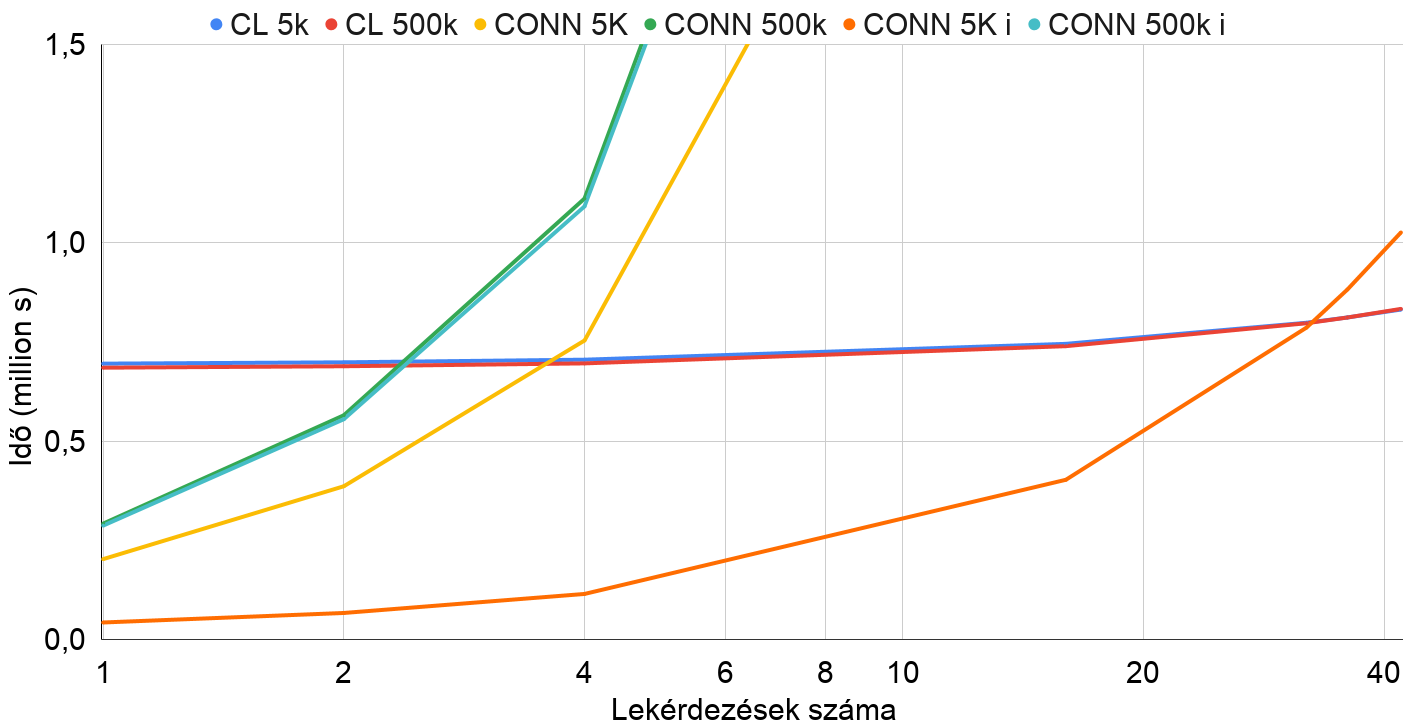
\includegraphics[width=\textwidth]{images/test/where3.png}
\caption{Becslés csak a lekérdezésre.}
\label{fig:where}
\end{figure}

\begin{figure}[h!]
\centering
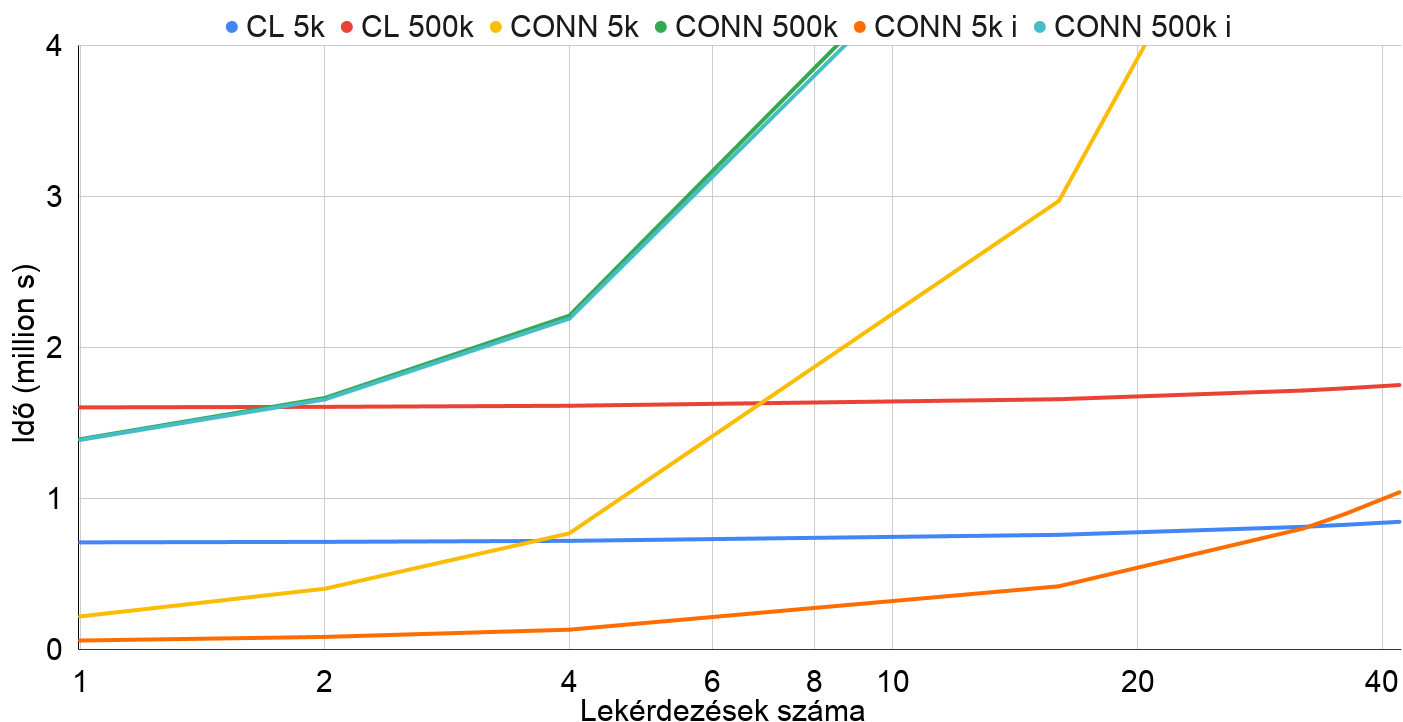
\includegraphics[width=\textwidth]{images/test/where_write3.png}
\caption{Becslés az eredmények kiírásával.}
\label{fig:where_write}
\end{figure}

A mérésekből a következő következtetéseket vonhatjuk le:
\begin{itemize}
	\item 0.5\% os visszatérési arany esetében ha nincs indexelés, akkor 7 lekérdezés után megtérülhetnek az \texttt{OpenCL} plusz költségei.
	\item Ha van indexelés abban az esetben ez a szám eléri a 37 -et.\newline
	50\% -os visszatérési aránynál már a 2. lekérdezésnél is nyereséges az \texttt{OpenCL} -es megvalósítás. 
\end{itemize}

\Aref{fig:where}. ábrán látható grafikonon a \texttt{CONN 500k} és \texttt{CONN 500k i} szinte egymást fedi, amiből látjuk, hogy ha a válaszban visszatérő sorok száma magas, akkor az indexelés hatékonysága alacsony.

\SubSection{Két táblás lekérdezés}
Forrás: programok, program\_test, join mappa.

Ehhez a részhez új adatbázist hoztam létre, az \texttt{EXPLAIN} bemutatásánál használthoz hasonlóan, de jelentősen nagyobb méretekkel, erre a tábla neve utal.
A generáláshoz szükséges kód megtalálható a \texttt{table gen} mappában.

\begin{python}
SELECT TM.c1p1, TS.c1p1, TM.c3 * TS.c3
FROM speed2.speed_262144 AS TM 
JOIN speed2.speed_131072 AS TS ON (TM.fk_s = TS.c1p1) 
WHERE TM.c3 > 9600 AND TS.c3 > 9200; 
	839 row(s) returned
...
WHERE TM.c3 > 9900 AND TS.c3 > 9900; 
	16 row(s) returned
\end{python}

A \texttt{Connector} mérési eredményei:

\begin{table}[h!]
\centering
\begin{tabular}{|p{6cm}|p{3cm}|p{3cm}|}
\hline
Sorok száma & 16 & 839 \\
\hline\hline

Előkészítés & $21425 \mu s$ & $21893 \mu s$ \\
\hline

Lekérdezés & 39363 $\mu s$ & 85889 $\mu s$ \\
\hline

Eredmény kiírás & 90 $\mu s$ & 2120 $\mu s$ \\
\hline

\end{tabular}
\end{table}

\newpage

Indexeléssel:

\begin{table}[h!]
\centering
\begin{tabular}{|p{6cm}|p{3cm}|p{3cm}|}
\hline
Sorok száma & 16 & 839 \\
\hline
\hline

Előkészítés & 20984 $\mu s$ & 26650 $\mu s$ \\
\hline

Lekérdezés & 10119 $\mu s$ & 31663 $\mu s$ \\
\hline

Eredmény kiírás & 97 $\mu s$ & 2802 $\mu s$ \\
\hline

\end{tabular}
\end{table}

OpenCL megvalósítás

\begin{table}[h!]
\centering
\begin{tabular}{|p{6cm}|p{3cm}|p{3cm}|}
\hline
Sorok száma & 16 & 839 \\
\hline
\hline
Előkészítés & 314073 $\mu s$ & 315964 $\mu s$ \\
\hline
Kernel 1. 2. futása & 559 $\mu s$ & 593 $\mu s$ \\
\hline
Kernel 3. futása & 7662 $\mu s$ & 103988 $\mu s$ \\
\hline
Eredmény kiolvasás & 1974 $\mu s$ & 1745 $\mu s$ \\
\hline
Eredmény kiírás & 161 $\mu s$ & 1932 $\mu s$ \\
\hline
\end{tabular}
\end{table}	

Az \texttt{OpenCL} -es futási időket igyekeztem optimalizálni azzal, hogy a szerverről csak a szükséges oszlopokat kértem le, így elkerülve a fölösleges adatok mozgatását.

\begin{figure}[h!]
\centering
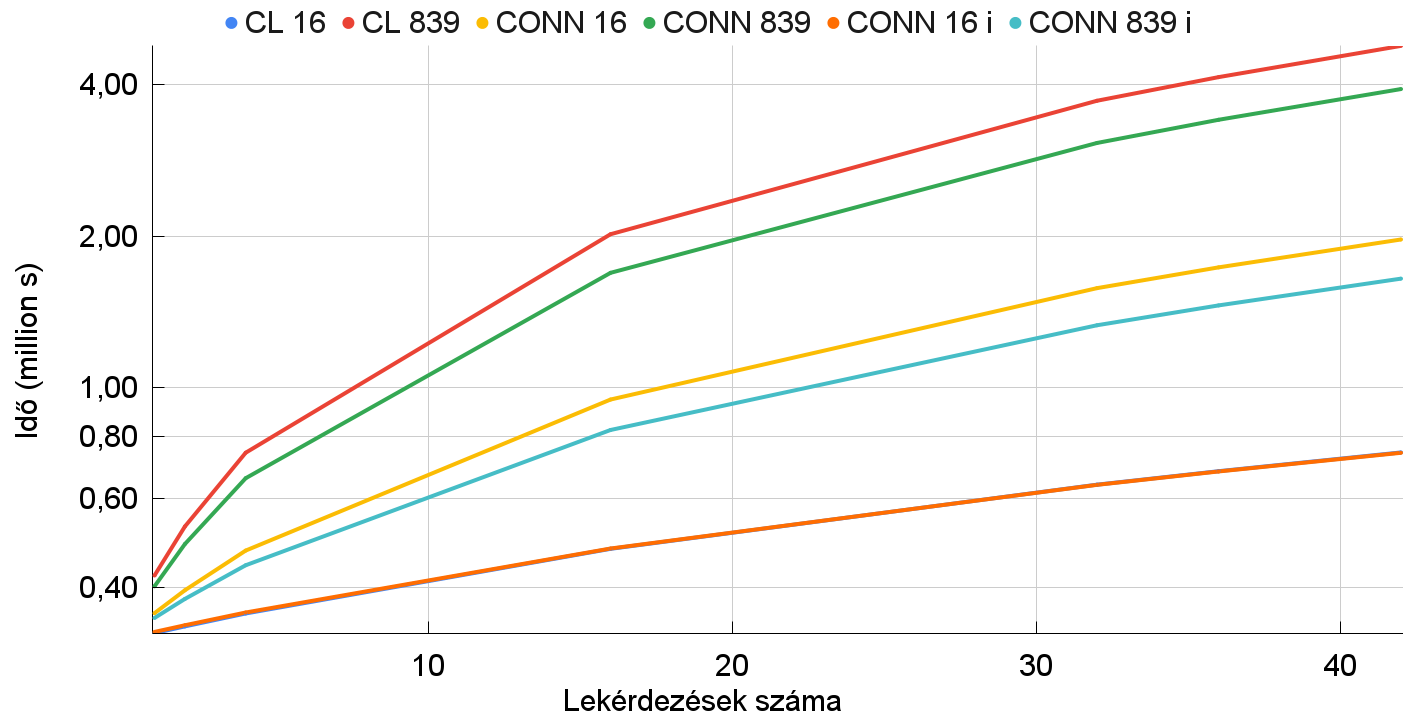
\includegraphics[width=\textwidth]{images/test/join2.png}
\caption{Becslés csak a lekérdezésre.}
\label{fig:join}
\end{figure}

\Aref{fig:join}. ábrán a méréseket látva, arra a következtetésre juthatunk, hogy az \texttt{OpenCL} program nem bizonyul hatékonynak, még ilyen alacsony találati számnál sem. A kiolvasási időt tovább lehetne optimalizálni az előzőekben említett másik módszerrel, ezzel akár tizedére is csökkenhet a kiolvasási idő, illetve minimálisan javulhat a kiírási idő is. Ez a kis számú lekérdezés annyira speciális esete lenne a lekérdezéseknek, hogy nem vizsgálom tovább.

A táblakapcsolás nélküli lekérdezéshez viszonyított drámai teljesítmény romlás oka az hogy a \texttt{MySQL} motorja a táblák kapcsolásánál felhasználja a másodlagos kulcsokat mint index így nem kell végignéznie minden sort a párokat keresve.

Valamilyen indexelési módszer használatával az \texttt{OpenCL} megvalósítás is optimalizálható lenne, ám ez bonyolult és költséges lehet.

A \Aref{fig:join} ábrán jól látható, hogy már 839 visszatérő sornál is a CL megvalósítás a leglassabb. A 16 soros lekérdezés pedig alig előzi meg az indexelt lekérdezést.
Az eredményekből azt is látjuk, hogy nagyobb mértékben nőtt a futási ideje a CL programnak, azaz még több visszatérő sor eseten a módszer még kevésbé hatékony.
